% A skeleton file for producing Computer Engineering reports
% https://github.com/DeepHorizons/KGCOEReport_template

\documentclass[CMPE]{KGCOEReport}

% The following should be changed to represent your personal information
\newcommand{\classCode}{CMPE 460}  % 4 char code with number
\newcommand{\name}{Jacob Meyerson}
\newcommand{\LabSectionNum}{2}
\newcommand{\LabInstructor}{Professor Beato}	
\newcommand{\TAs}{Brunon Sztuba \\ Eri Montano \\ Connor Henley}
\newcommand{\LectureSectionNum}{1}
\newcommand{\LectureInstructor}{Professor Beato}
\newcommand{\exerciseNumber}{7}
\newcommand{\exerciseDescription}{Filter Design and Simulation}
\newcommand{\dateDone}{March 26, 2021}
\newcommand{\dateSubmitted}{April 2, 2021}

\usepackage{float}
\usepackage{titlesec}
\usepackage{pdfpages}
\usepackage{siunitx}

\begin{document}
\maketitle

\iffalse % No table of contents or other sections for a worksheet -------------------------------------------------
\tableofcontents	%Make a table of contents for all of the sections
\newpage			%New page after table of contents

%Abstract Section
\section*{Abstract}
\addcontentsline{toc}{section}{Abstract}
		
%Design Methodology Section
\section*{Design Methodology}
\addcontentsline{toc}{section}{Design Methodology}

%Results Section	
\section*{Results \& Analysis}
\addcontentsline{toc}{section}{Results \& Analysis}

%Conclusion Section
\section*{Conclusion}
\addcontentsline{toc}{section}{Conclusion}

\fi % -------------------------------------------------------------------------------------------------------------------------------

\section*{Lab Description}
This lab explored different types of low pass filters by using LTSpice to design and simulate active and passive filters. In addition, a three op amp biquad band pass filter was designed and simulated. The purpose of this exercise was to solve for different circuit components to simulate passive and active filters with desired specifications like cutoff frequency or center frequency. This exercise was successful because all filters simulated performed with their design requirements in simulations. 

\section*{Circuit Schematics and Graphs}
\subsection*{First Order RC Passive Low Pass Filter}

\begin{figure}[H]
	\centering
  	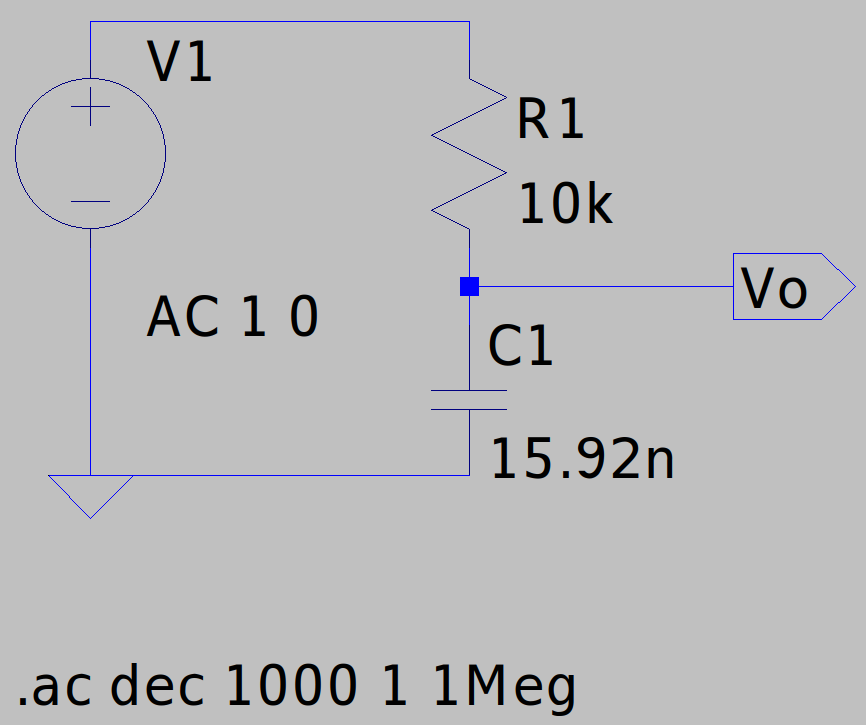
\includegraphics[width=0.45\textwidth]{Screenshots/q2_schematic}  
	\caption{First Order Passive LPF Schematic with $f_c = 1 \si{\kilo\hertz}$}
	\label{q2_schematic}
\end{figure}

\begin{figure}[H]
	\centering
  	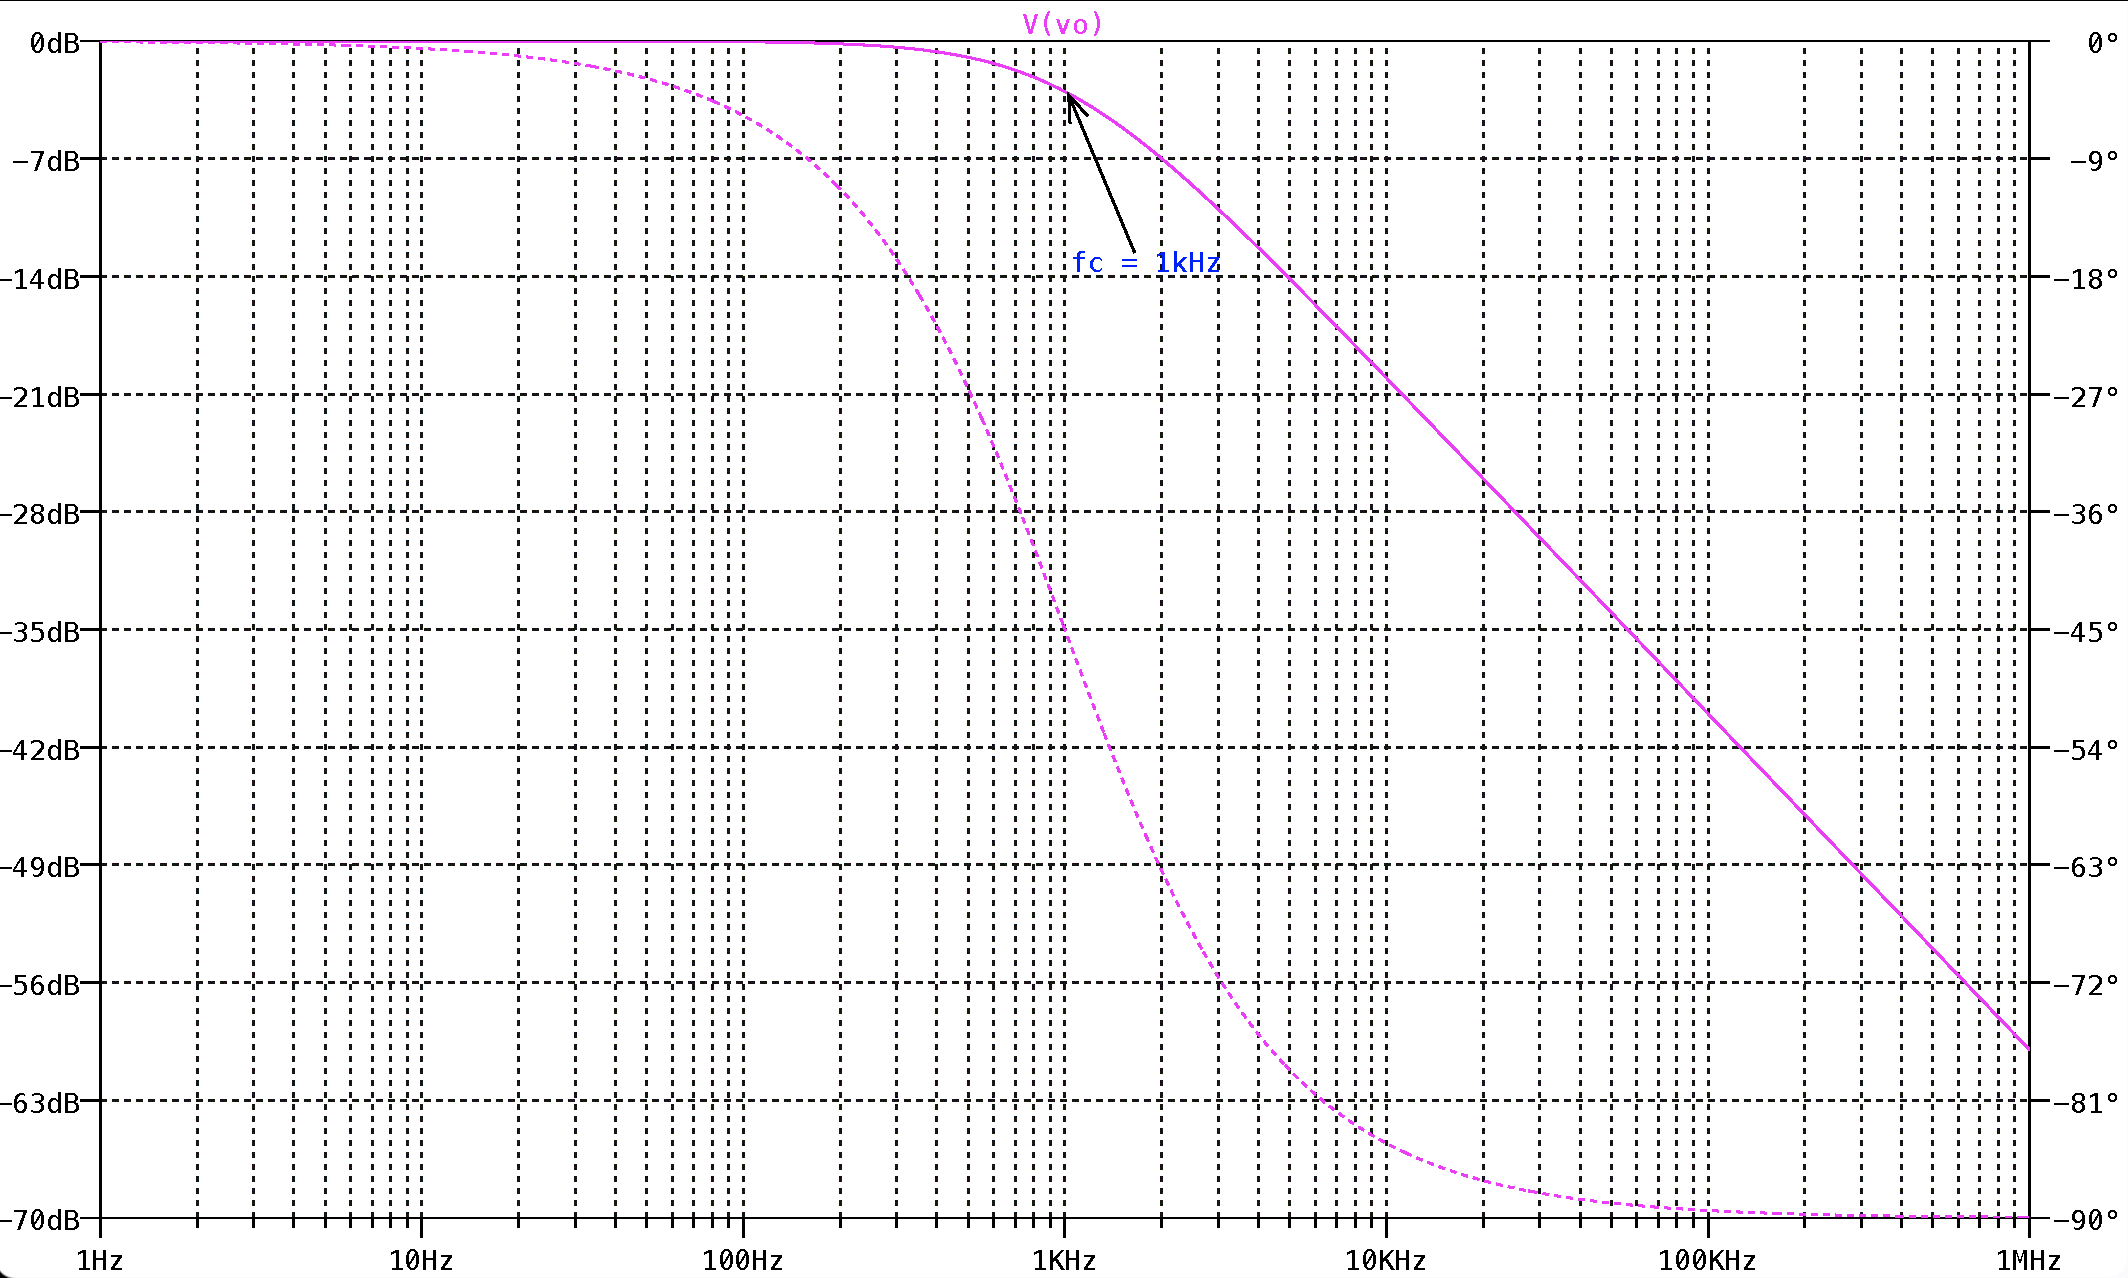
\includegraphics[width=0.65\textwidth]{Screenshots/q2_graph}  
	\caption{First Order Passive LPF Graph with $f_c = 1 \si{\kilo\hertz}$}
	\label{q2_graph}
\end{figure}

\begin{figure}[H]
	\centering
  	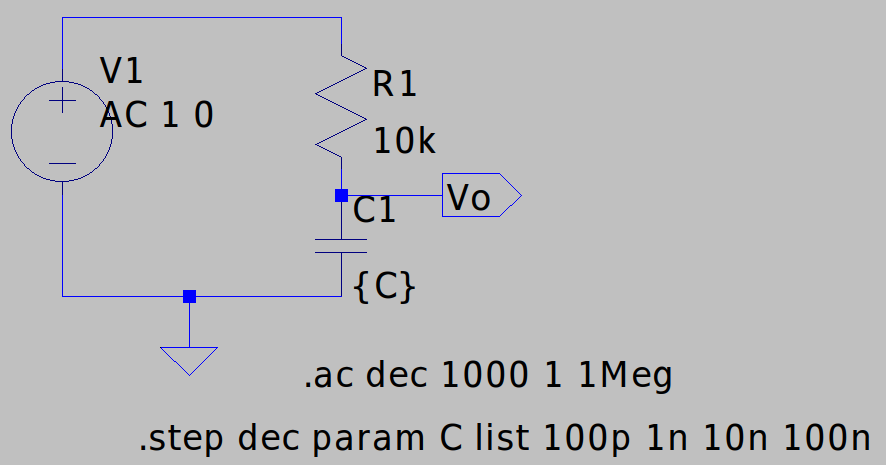
\includegraphics[width=0.45\textwidth]{Screenshots/q3_schematic}  
	\caption{First Order Passive LPF Schematic with Capacitor Sweep}
	\label{q3_schematic}
\end{figure}

%Figure \ref{q3_graph} shows the magnitude and phase plots for the AC parametric sweep done on Figure \ref{q3_schematic}. The solid lines all represent the magnitudes, and the dashed lines all represent the phase. The red lines correspond to a capacitor value of 100 nF. The blue lines correspond to the capacitor value of 10 nF. The green lines correspond to the capacitor value of 1 nF, and the pink lines correspond to the capacitor value of 100 pF. As shown in the graph, the cutoff frequencies for the list of capacitors, 100 pF, 1 nF, 10 nF, 100 nF are 159.155 kHz, 15.9155 kHz, 1.59155 kHz, and .159155 kHz, respectively. The slopes of all magnitude plots decrease at a rate of -20 db/dec.

\begin{figure}[H]
	\centering
  	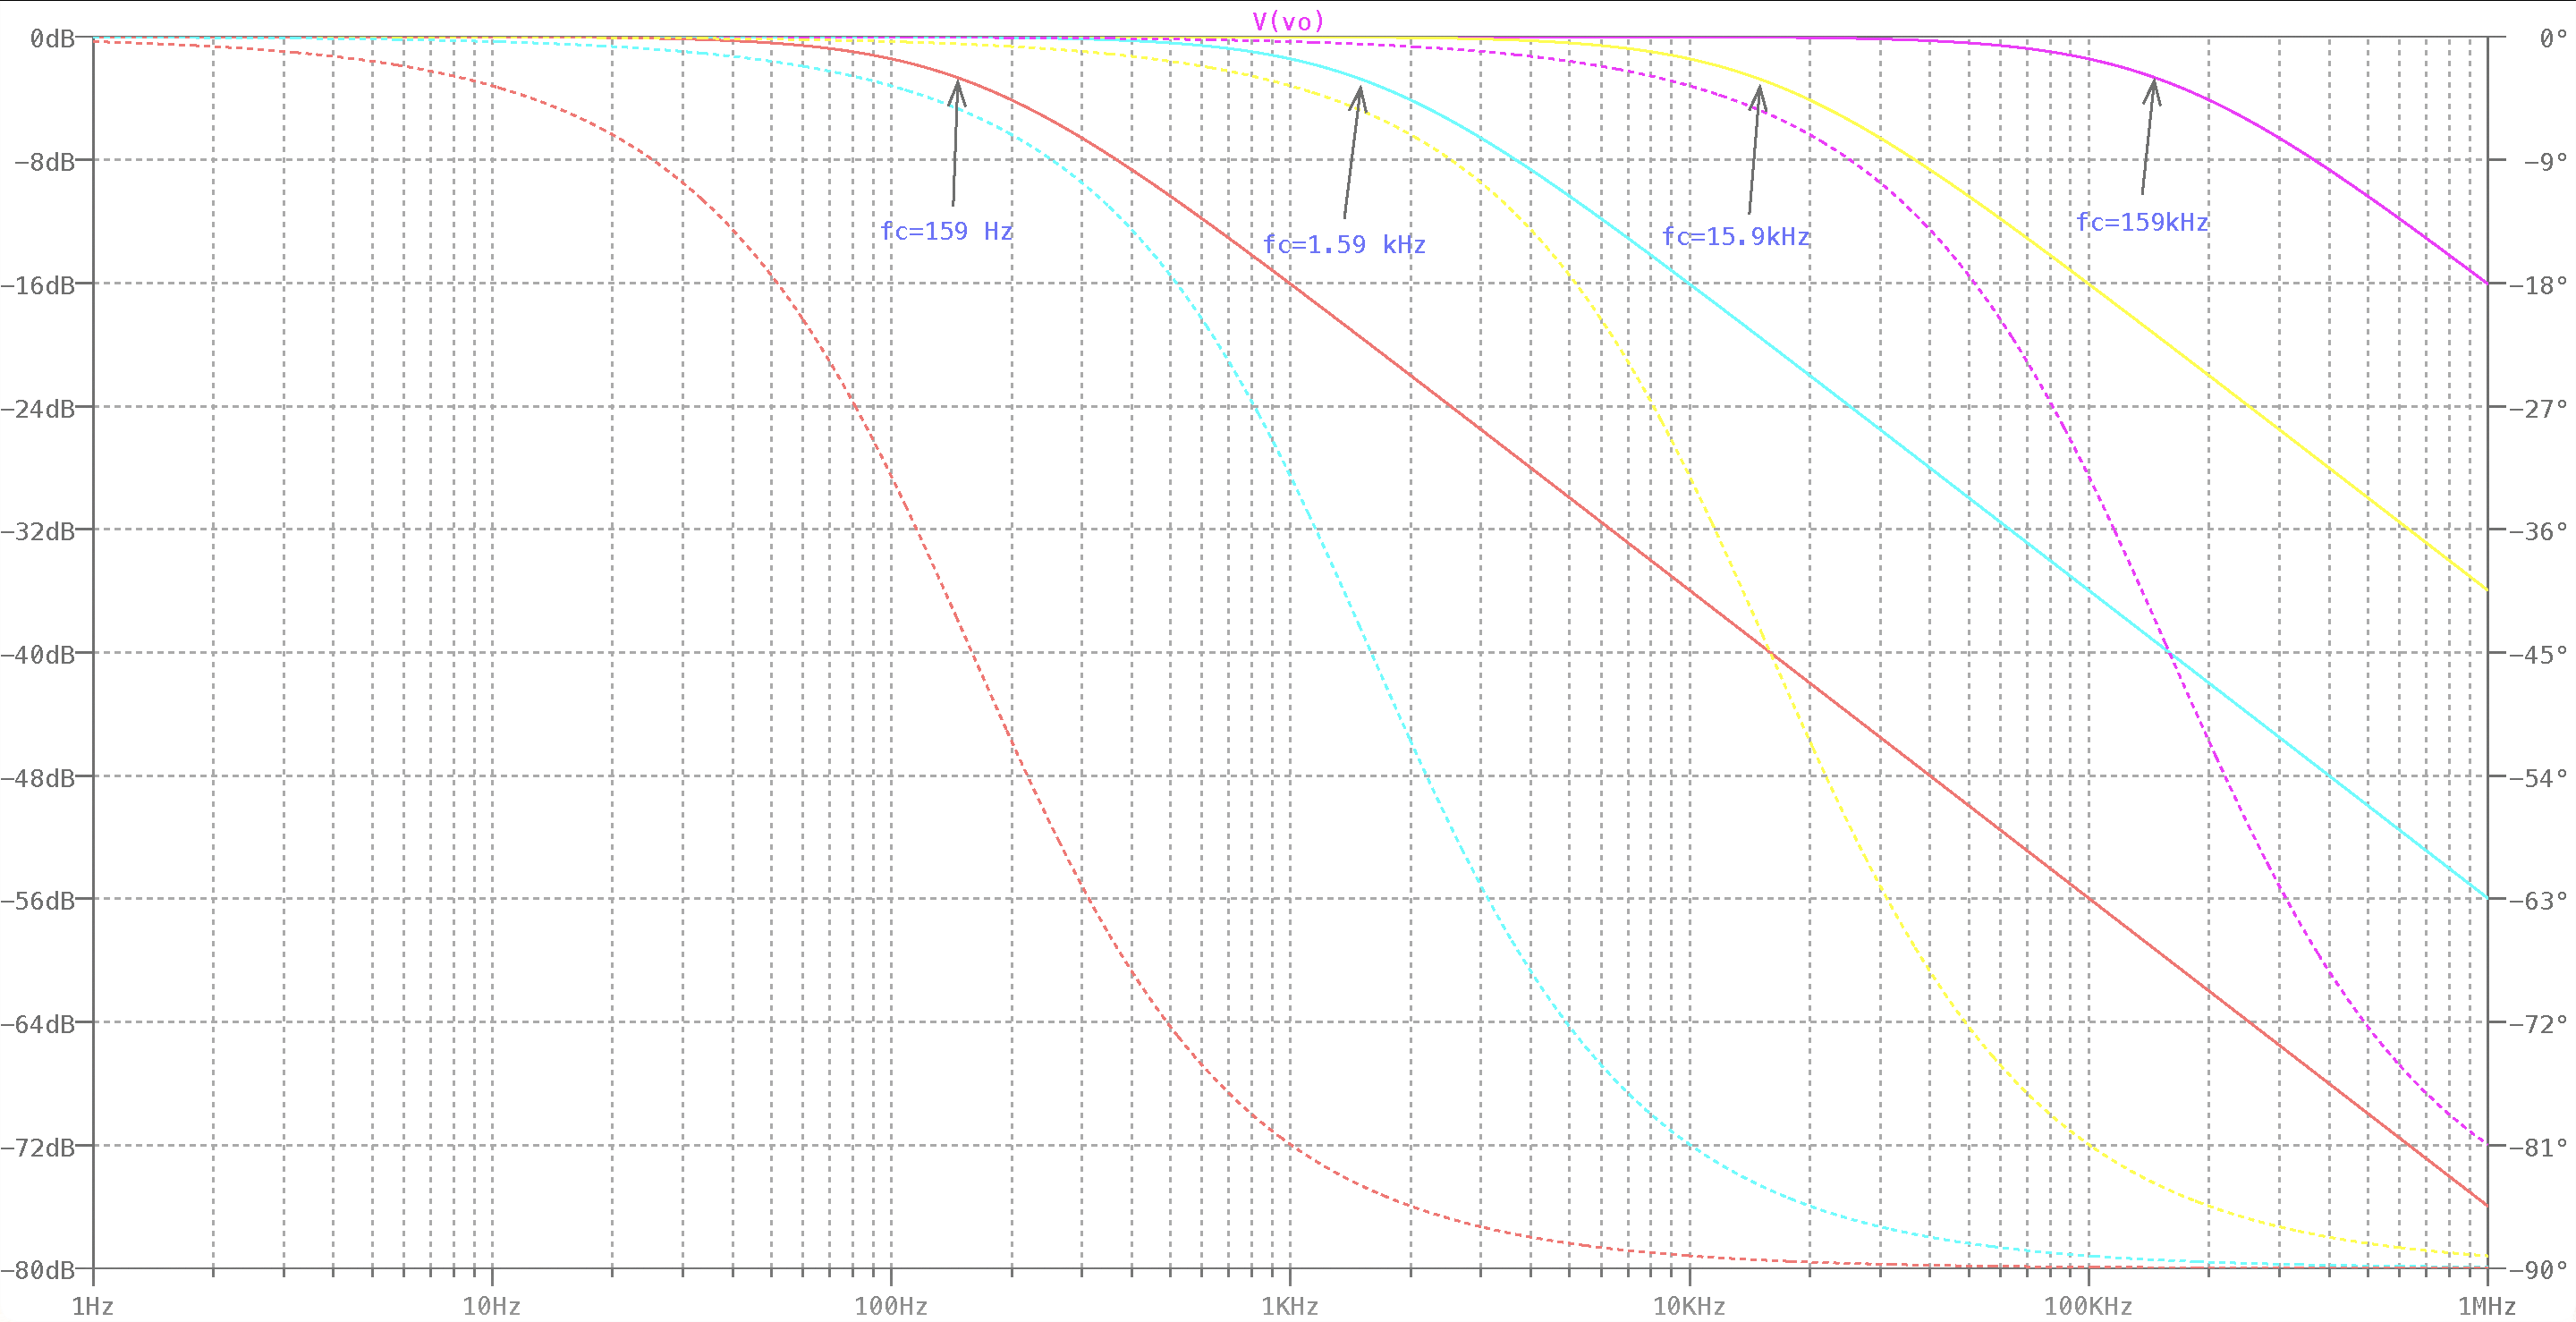
\includegraphics[width=0.65\textwidth]{Screenshots/q3_graph}  
	\caption{First Order Passive LPF Graph with Capacitor Sweep}
	\label{q3_graph}
\end{figure}

\subsection*{First, Second and Third Order RC Passive Low Pass Filter}

\begin{figure}[H]
	\centering
  	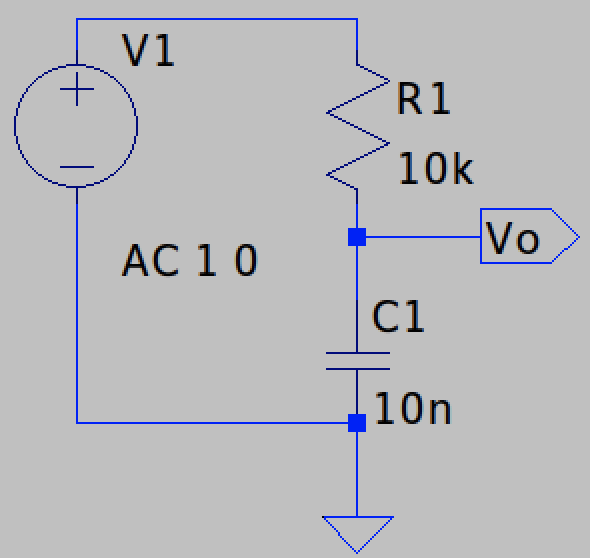
\includegraphics[width=0.45\textwidth]{Screenshots/q4_first_order_schematic}  
	\caption{First Order Passive LPF Schematic}
	\label{q4_schematic_1}
\end{figure}

\begin{figure}[H]
	\centering
  	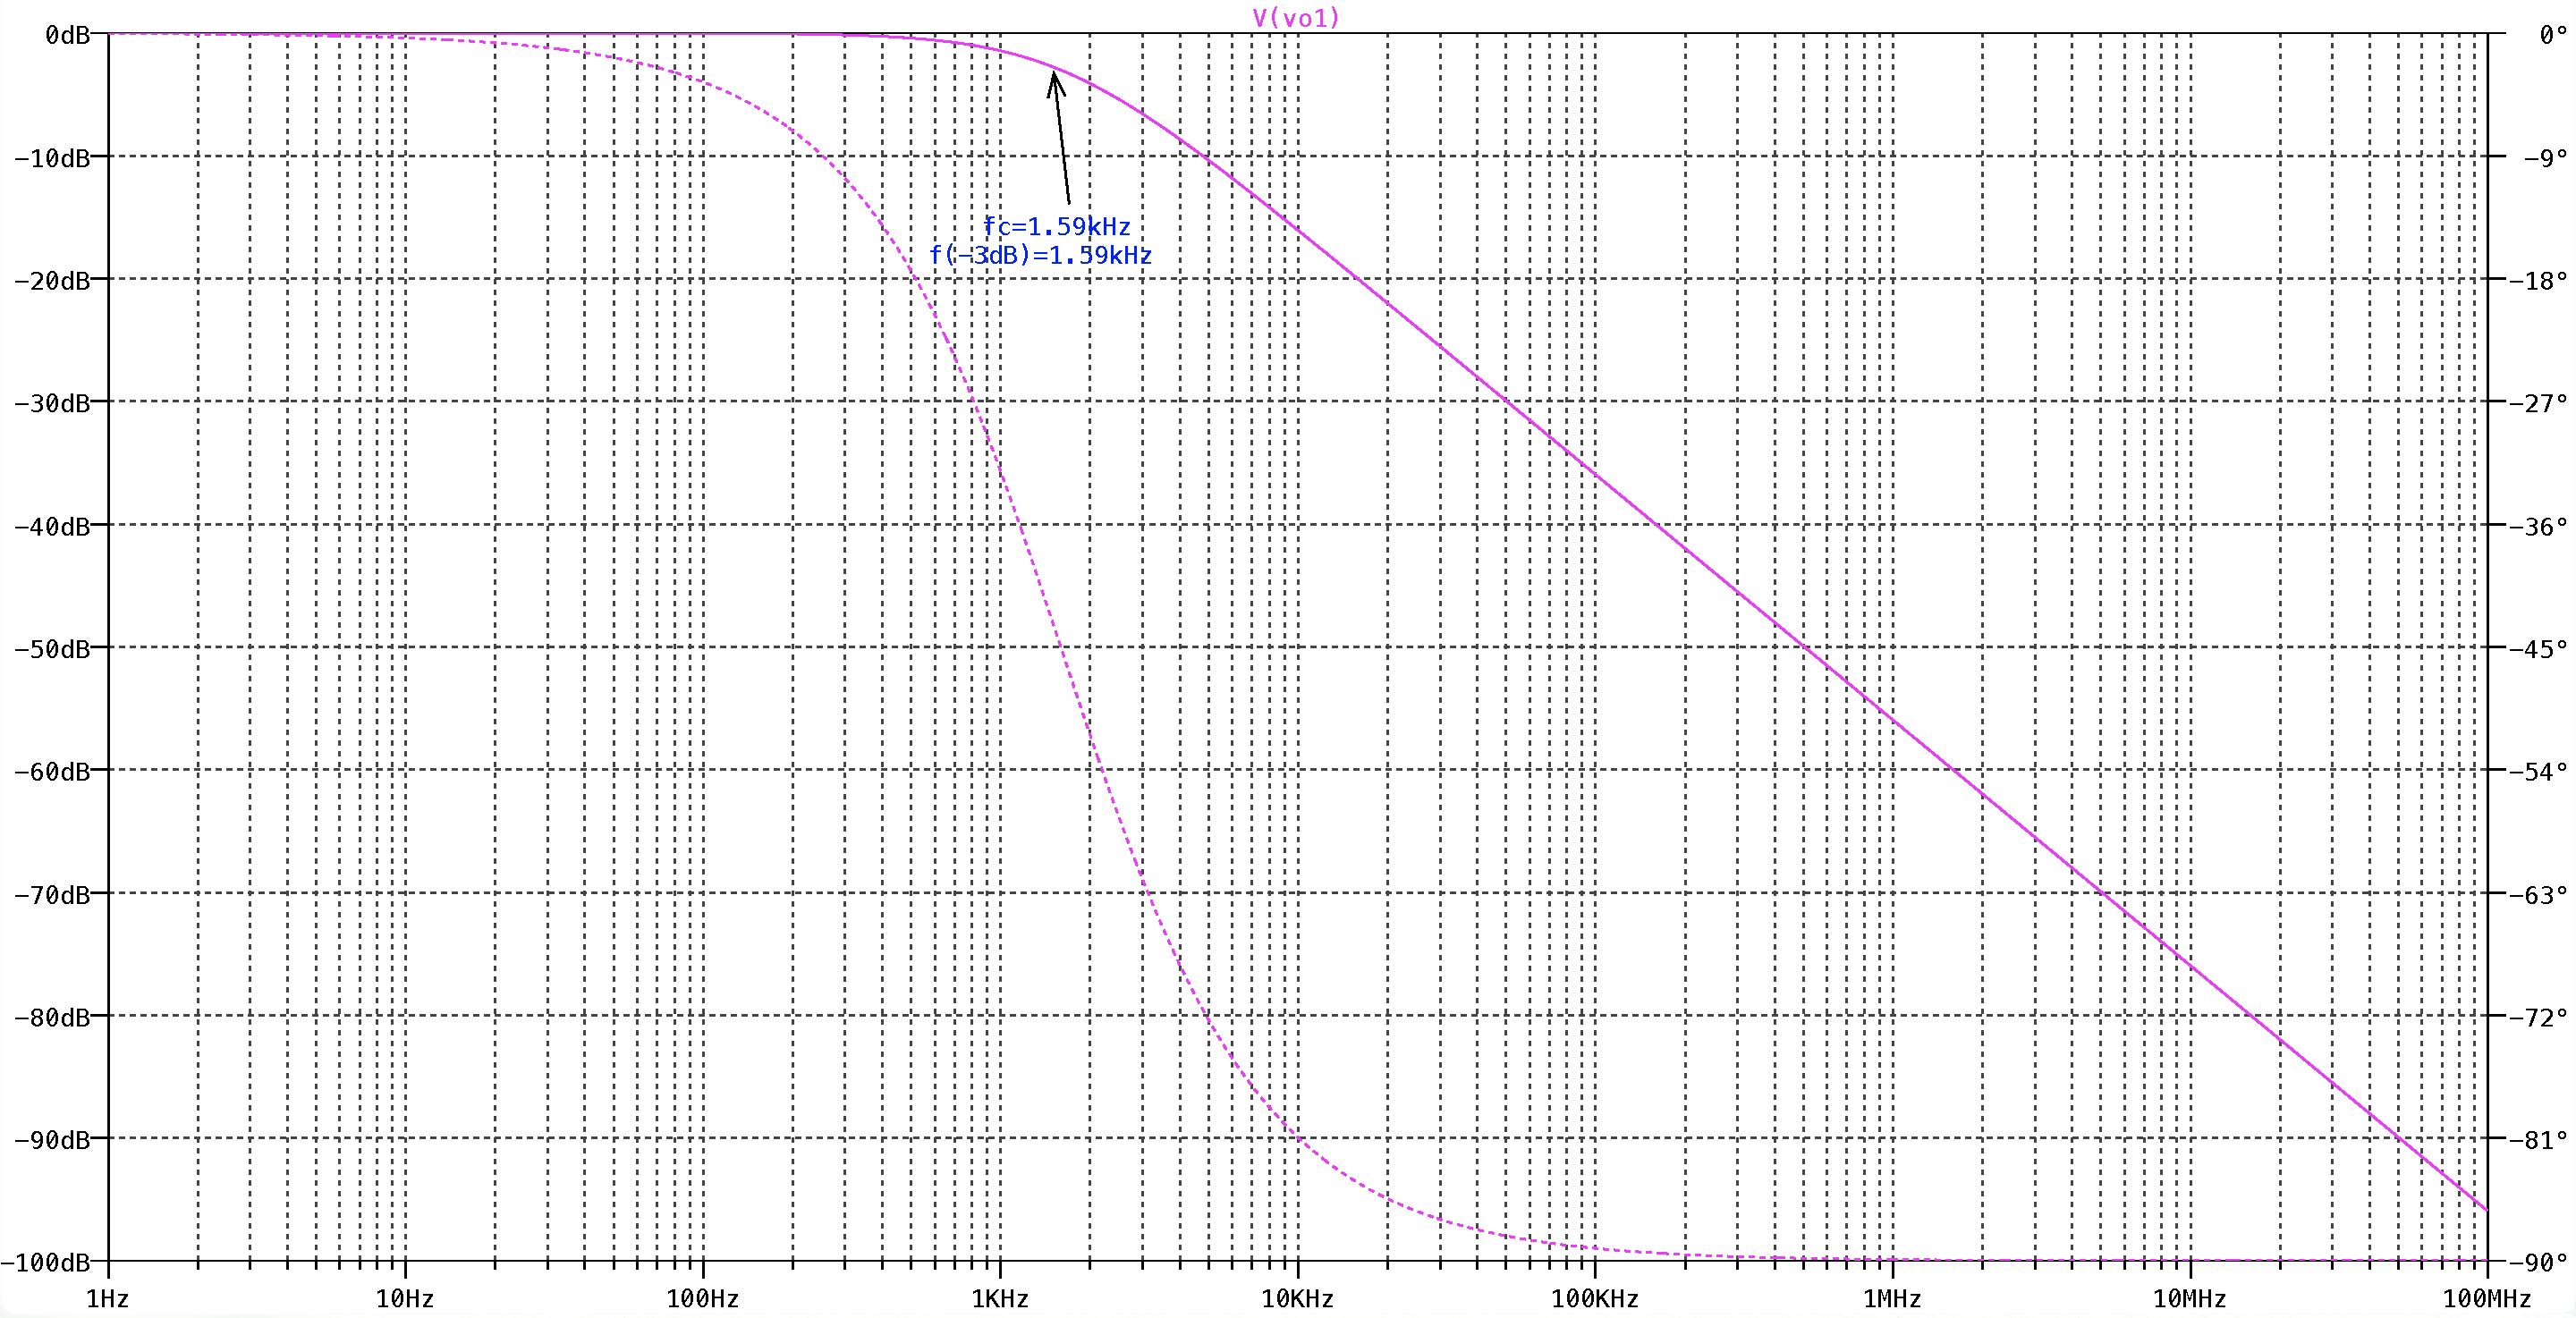
\includegraphics[width=0.65\textwidth]{Screenshots/q4_first_order_graph}  
	\caption{First Order Passive LPF Graph}
	\label{q4_graph_1}
\end{figure}

\begin{figure}[H]
	\centering
  	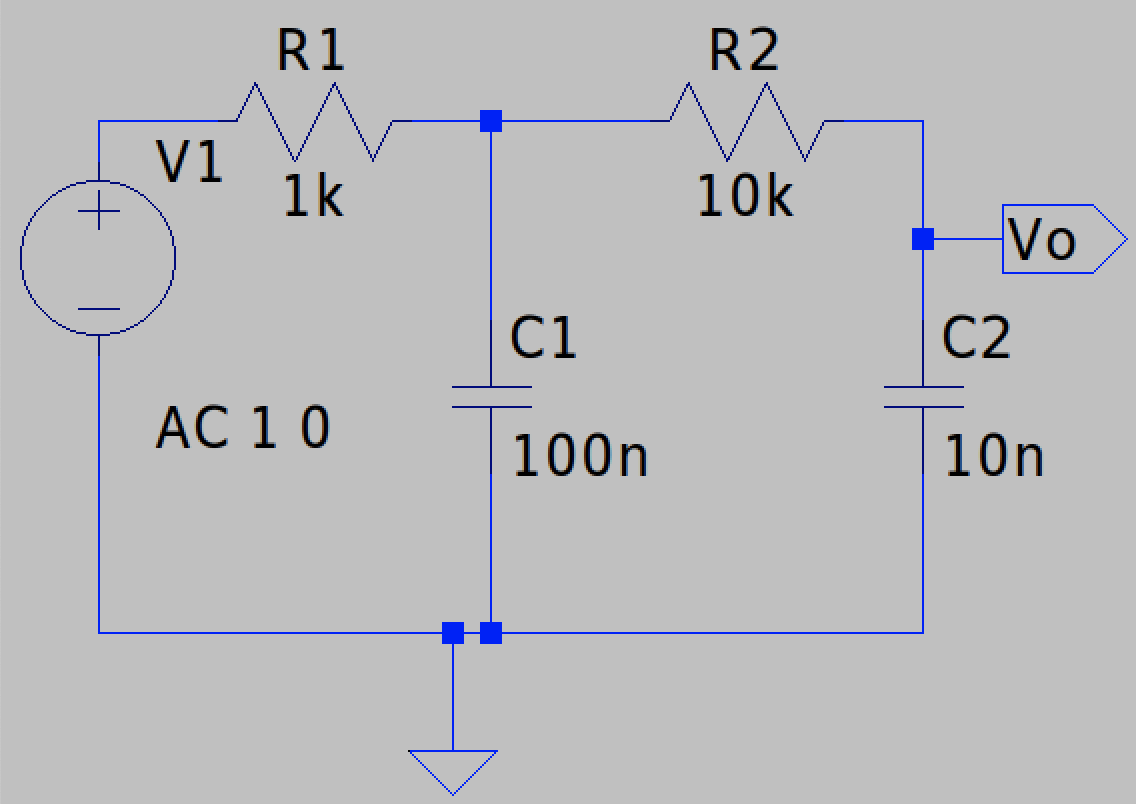
\includegraphics[width=0.45\textwidth]{Screenshots/q4_second_order_schematic}  
	\caption{Second Order Passive LPF Schematic}
	\label{q4_schematic_2}
\end{figure}

\begin{figure}[H]
	\centering
  	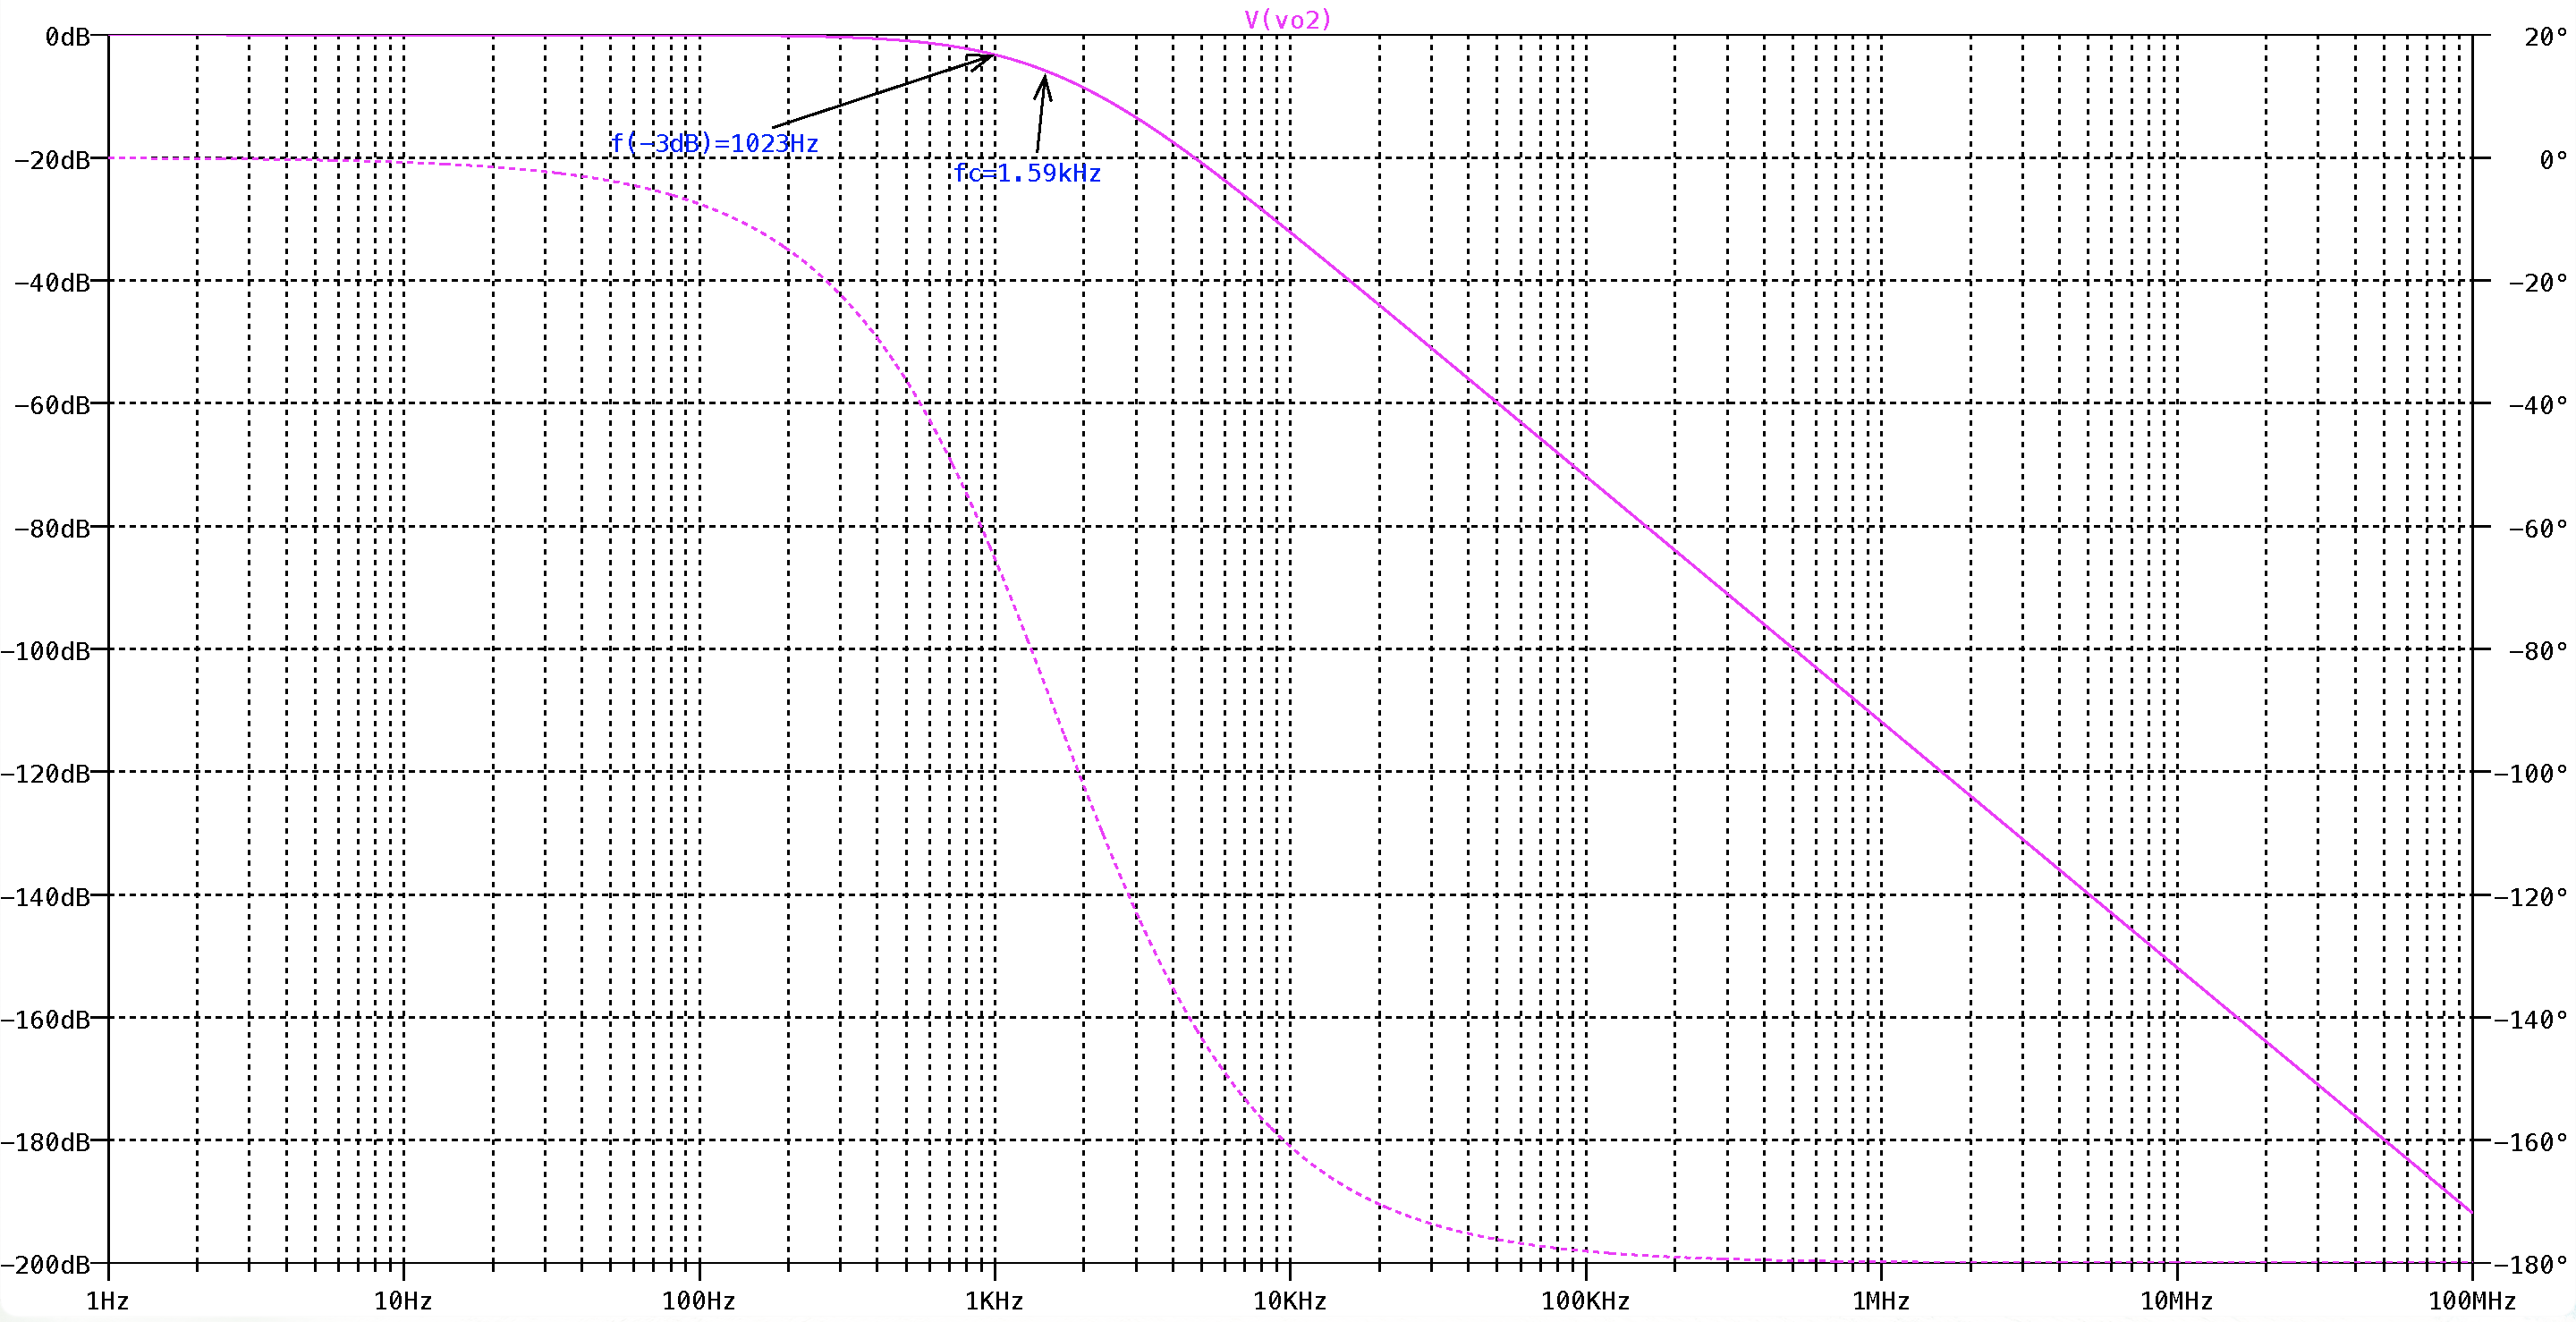
\includegraphics[width=0.65\textwidth]{Screenshots/q4_second_order_graph}  
	\caption{Second Order Passive LPF Graph}
	\label{q4_graph_2}
\end{figure}

\begin{figure}[H]
	\centering
  	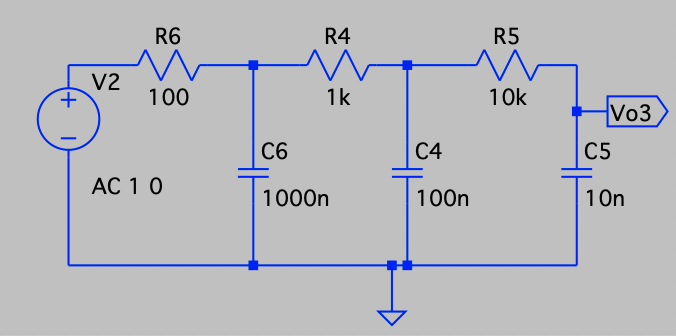
\includegraphics[width=0.45\textwidth]{Screenshots/q4_third_order_schematic}  
	\caption{Third Order Passive LPF Schematic}
	\label{q4_schematic_3}
\end{figure}

\begin{figure}[H]
	\centering
  	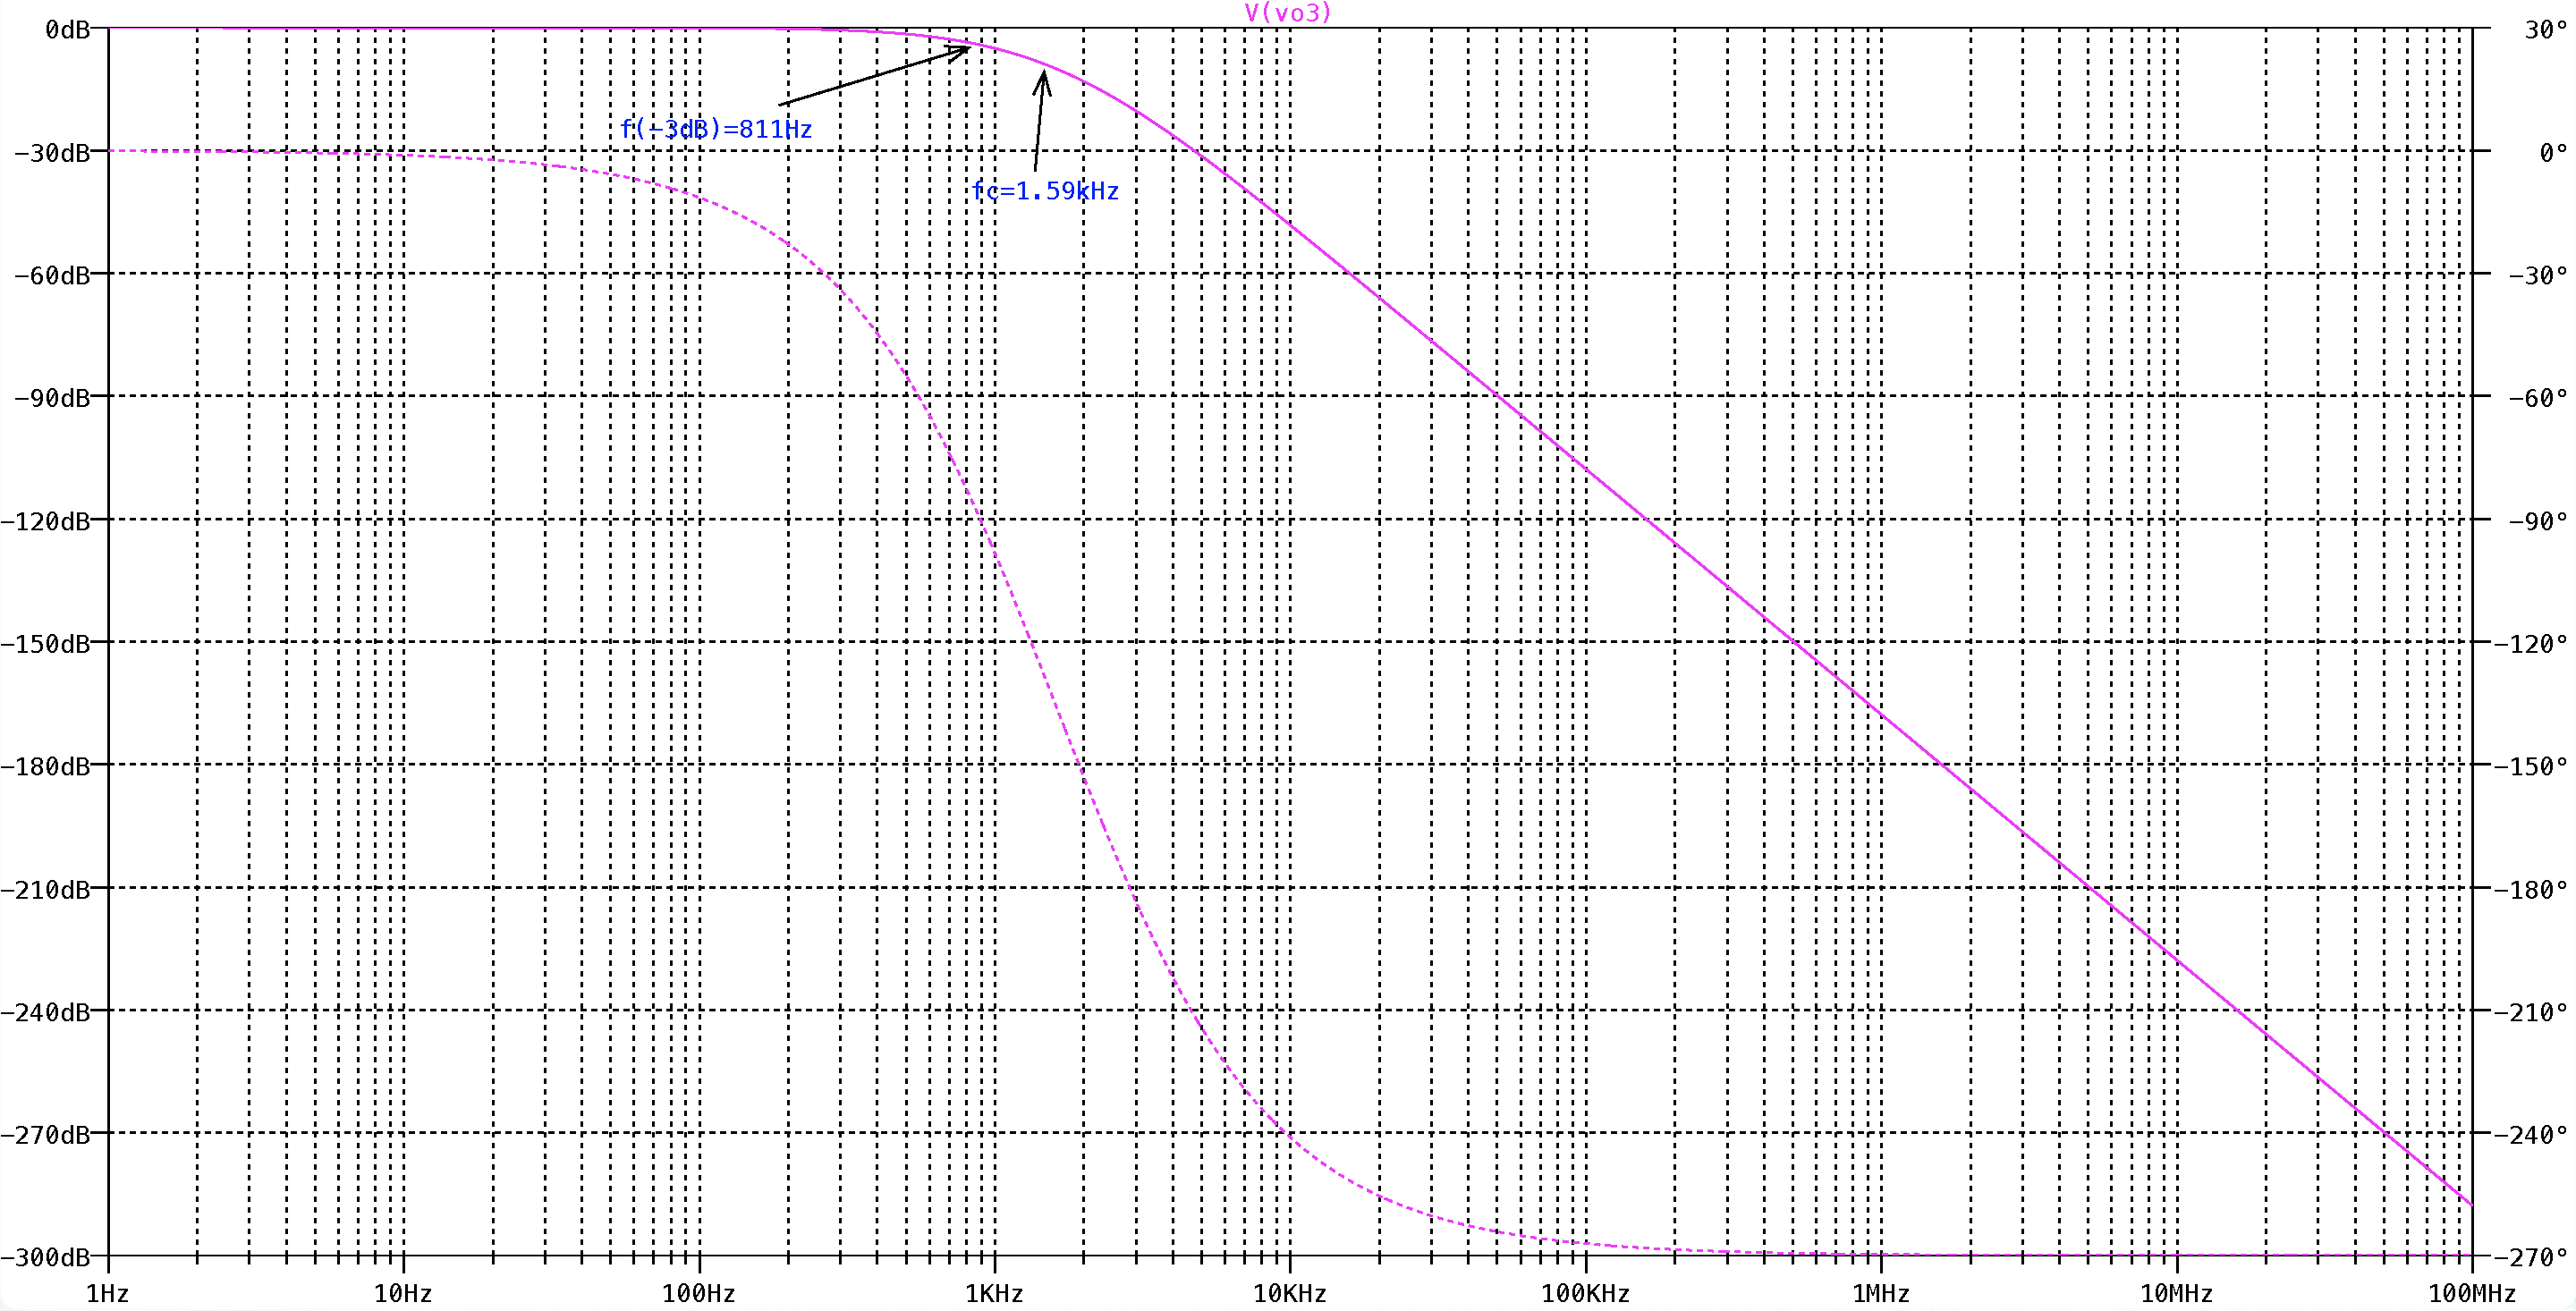
\includegraphics[width=0.65\textwidth]{Screenshots/q4_third_order_graph}  
	\caption{Third Order Passive LPF Graph}
	\label{q4_graph_3}
\end{figure}

\subsection*{Sallen-Key Second Order Low Pass Filter}

\begin{figure}[H]
	\centering
  	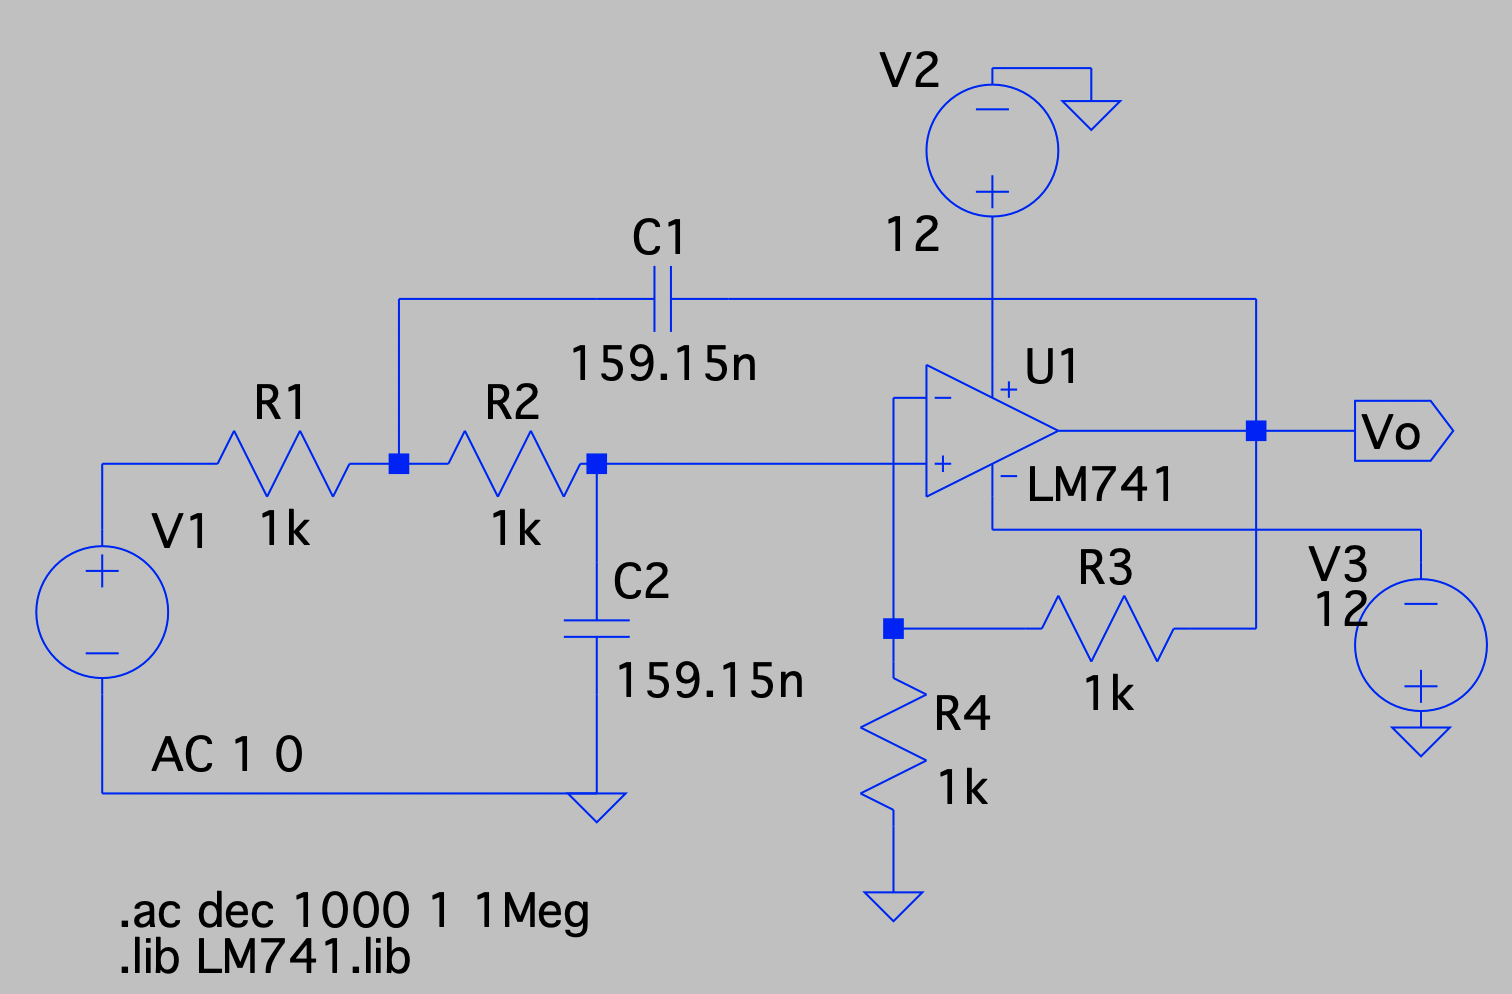
\includegraphics[width=0.45\textwidth]{Screenshots/q5_schematic}  
	\caption{Sallen Key Second Order LPF Schematic}
	\label{q5_schematic}
\end{figure}

\begin{figure}[H]
	\centering
  	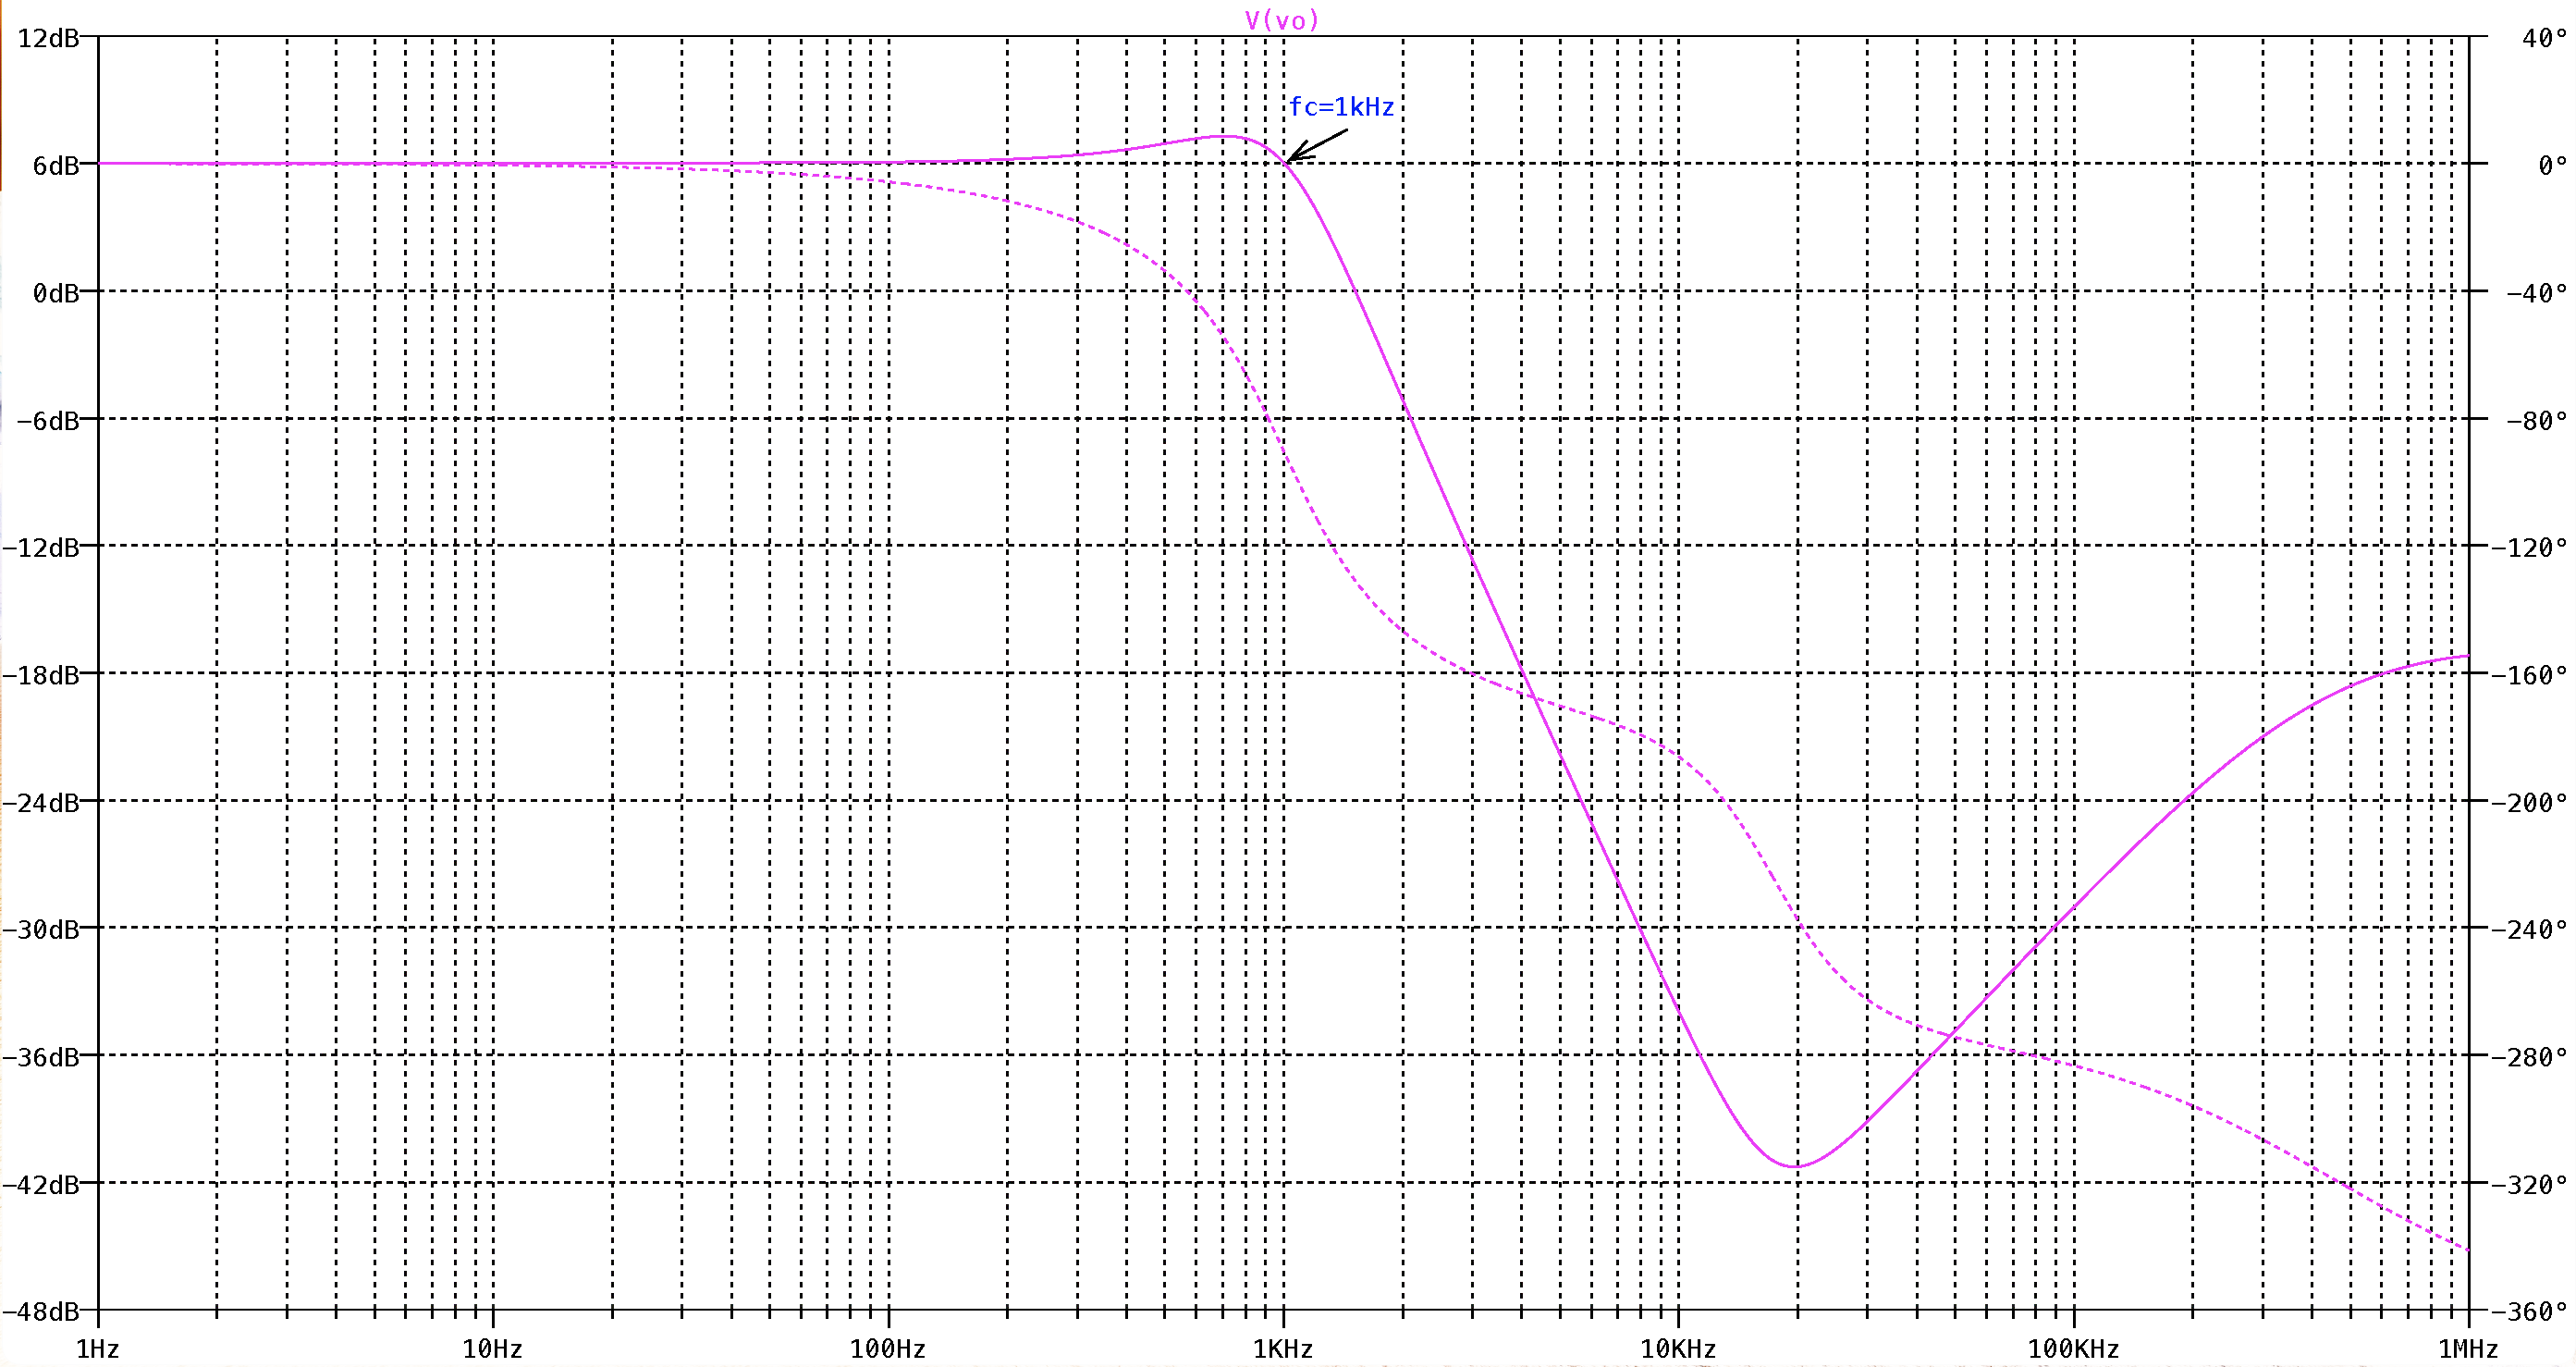
\includegraphics[width=0.65\textwidth]{Screenshots/q5_graph}  
	\caption{Sallen Key Second Order LPF Graph}
	\label{q5_graph}
\end{figure}

\subsection*{One Op-Amp Second Order VCVS Low Pass Filter (Butterworth Filter)}

\begin{figure}[H]
	\centering
  	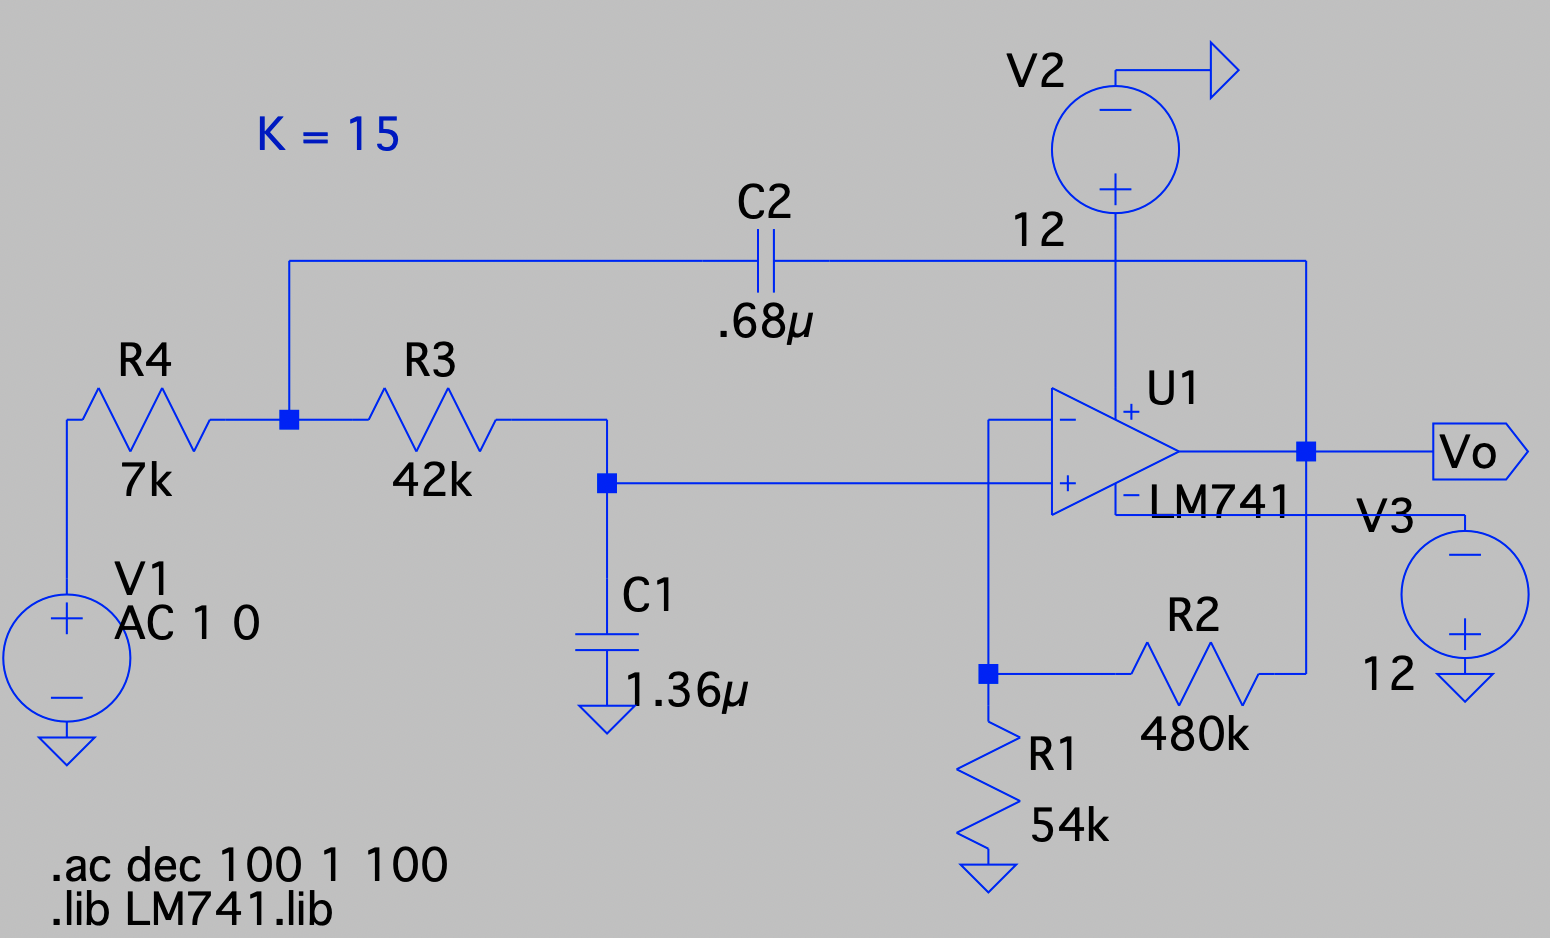
\includegraphics[width=0.45\textwidth]{Screenshots/q6_schematic}  
	\caption{Butterworth LPF Schematic}
	\label{q6_schematic}
\end{figure}

\begin{figure}[H]
	\centering
  	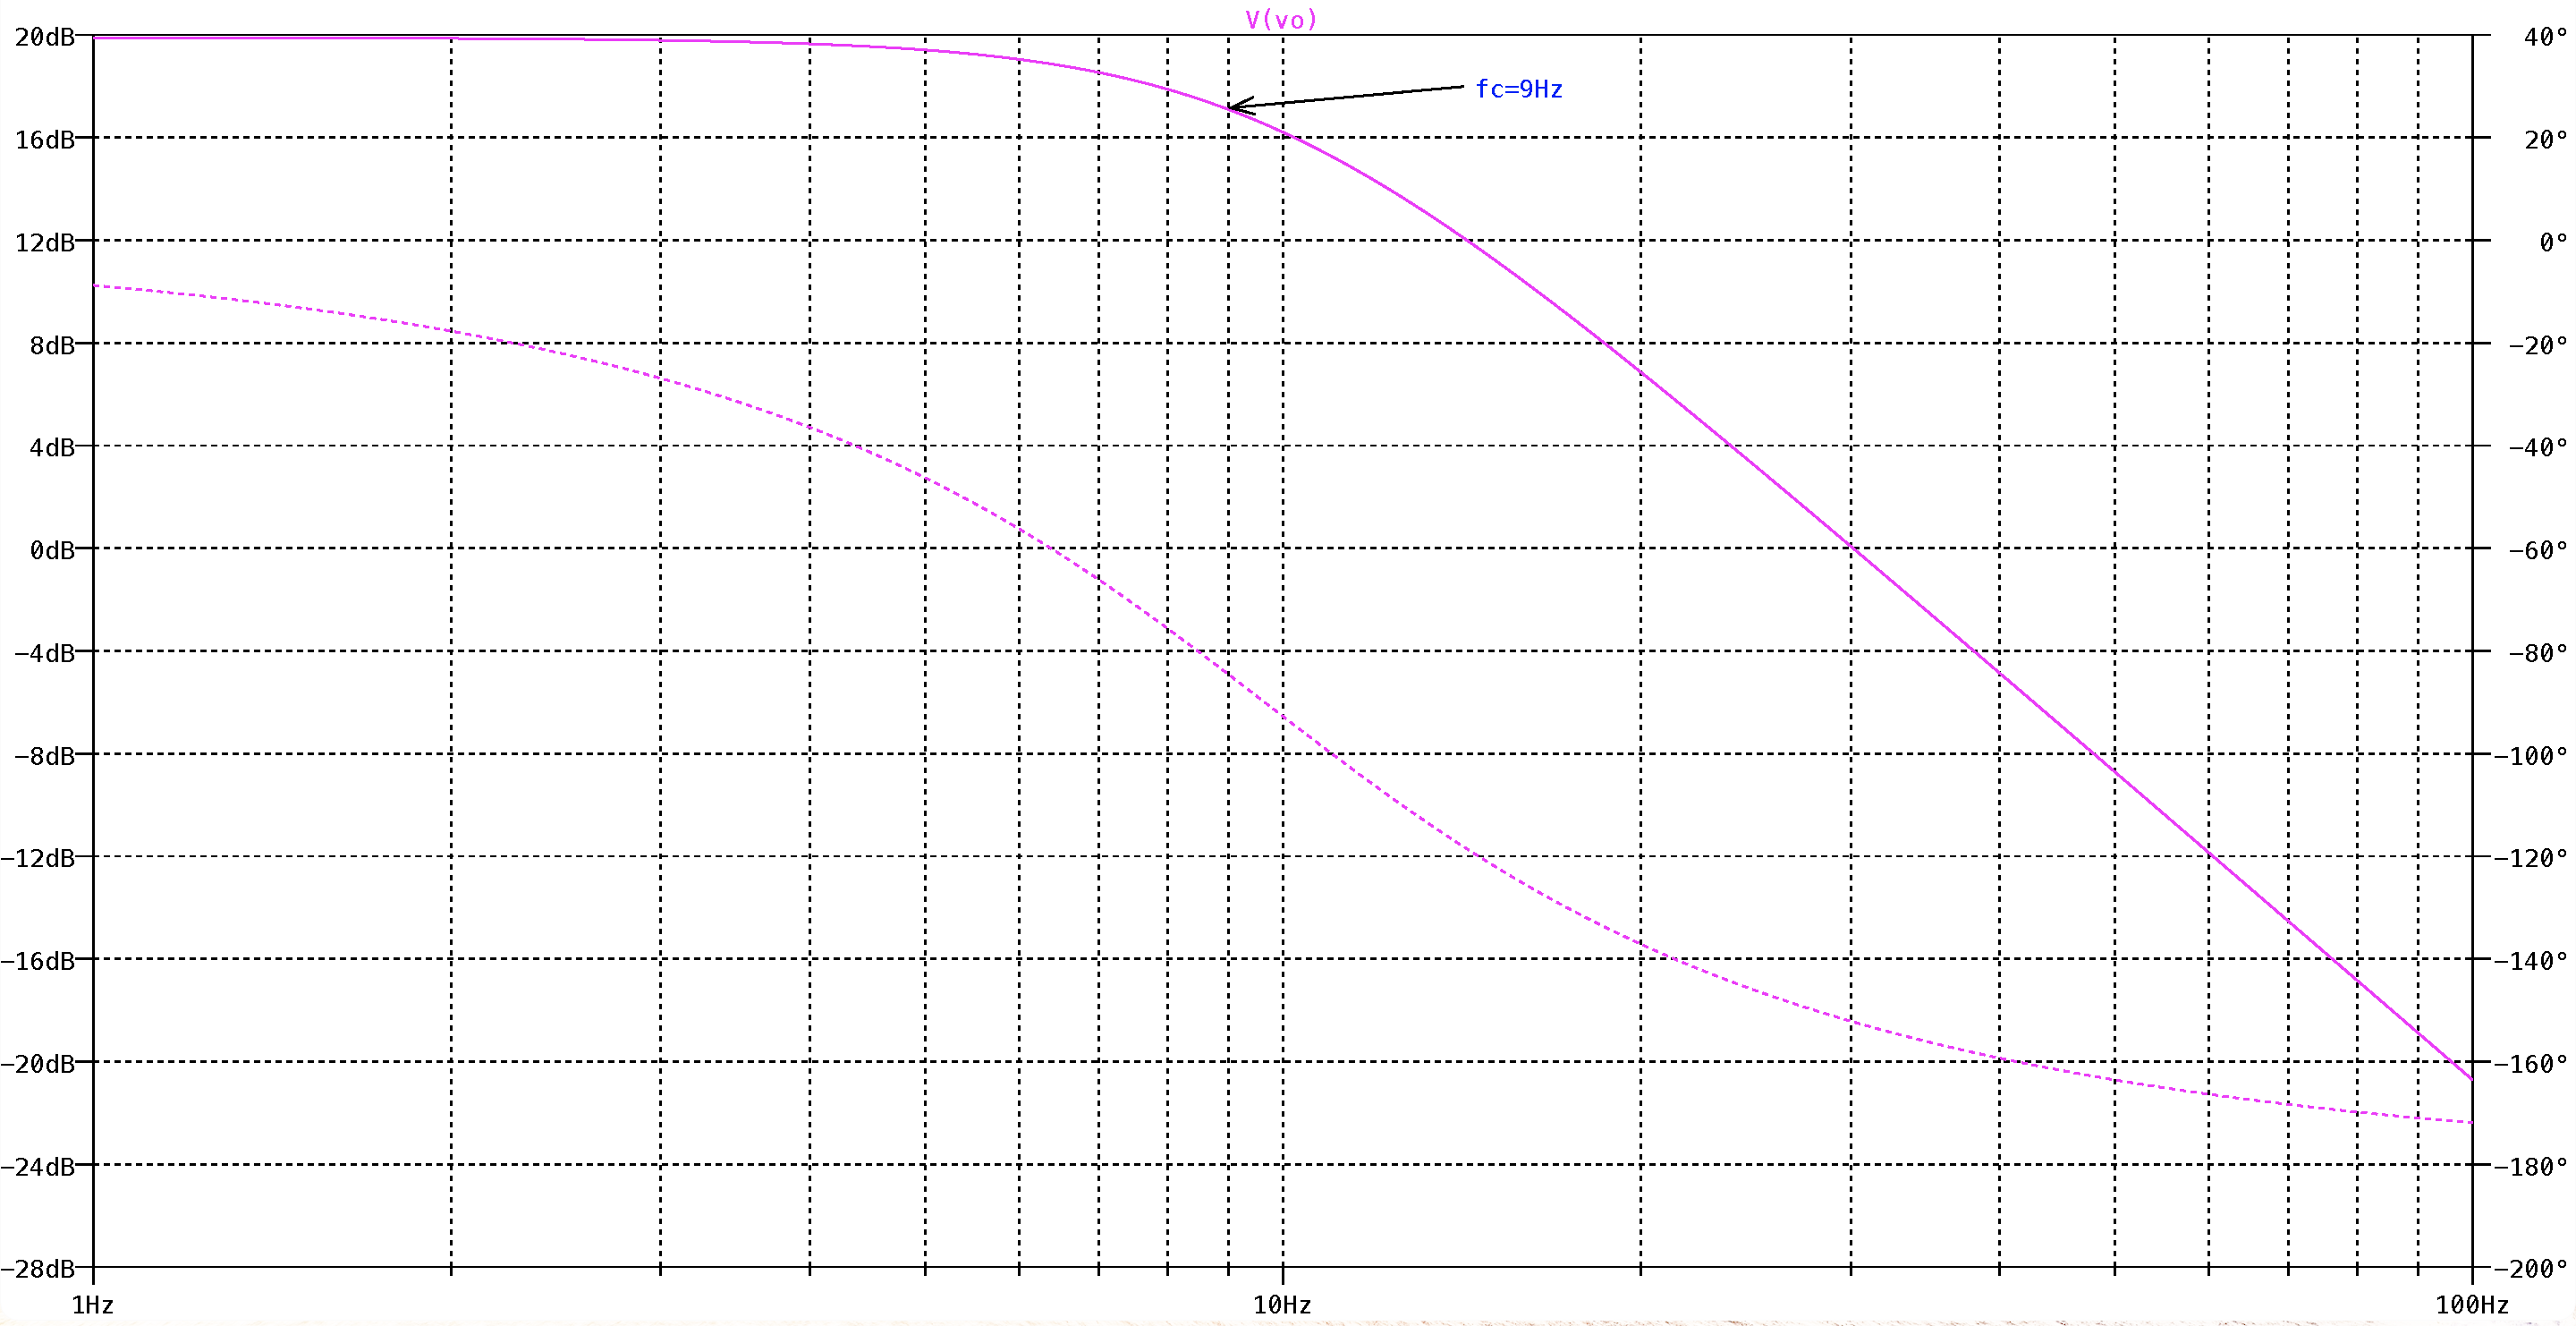
\includegraphics[width=0.65\textwidth]{Screenshots/q6_graph}  
	\caption{Butterworth LPF Graph}
	\label{q6_graph}
\end{figure}

\subsection*{Three Op-Amp Biquad Band Pass Filter}

\begin{figure}[H]
	\centering
  	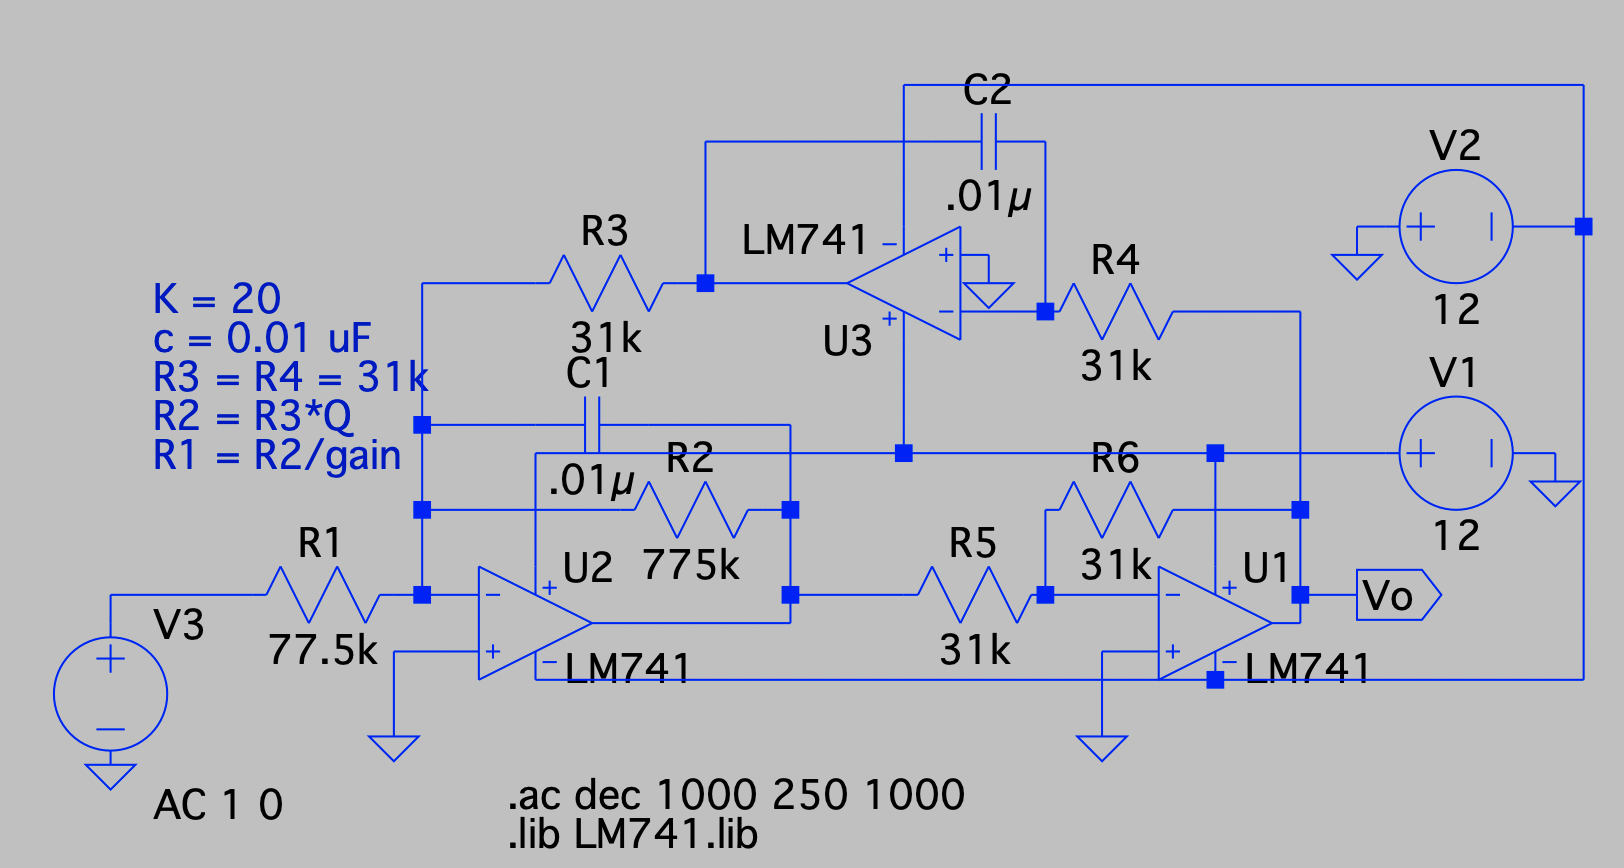
\includegraphics[width=0.45\textwidth]{Screenshots/q7_schematic}  
	\caption{Three Op-Amp Biquad Band Pass Filter Schematic}
	\label{q6_schematic}
\end{figure}

\begin{figure}[H]
	\centering
  	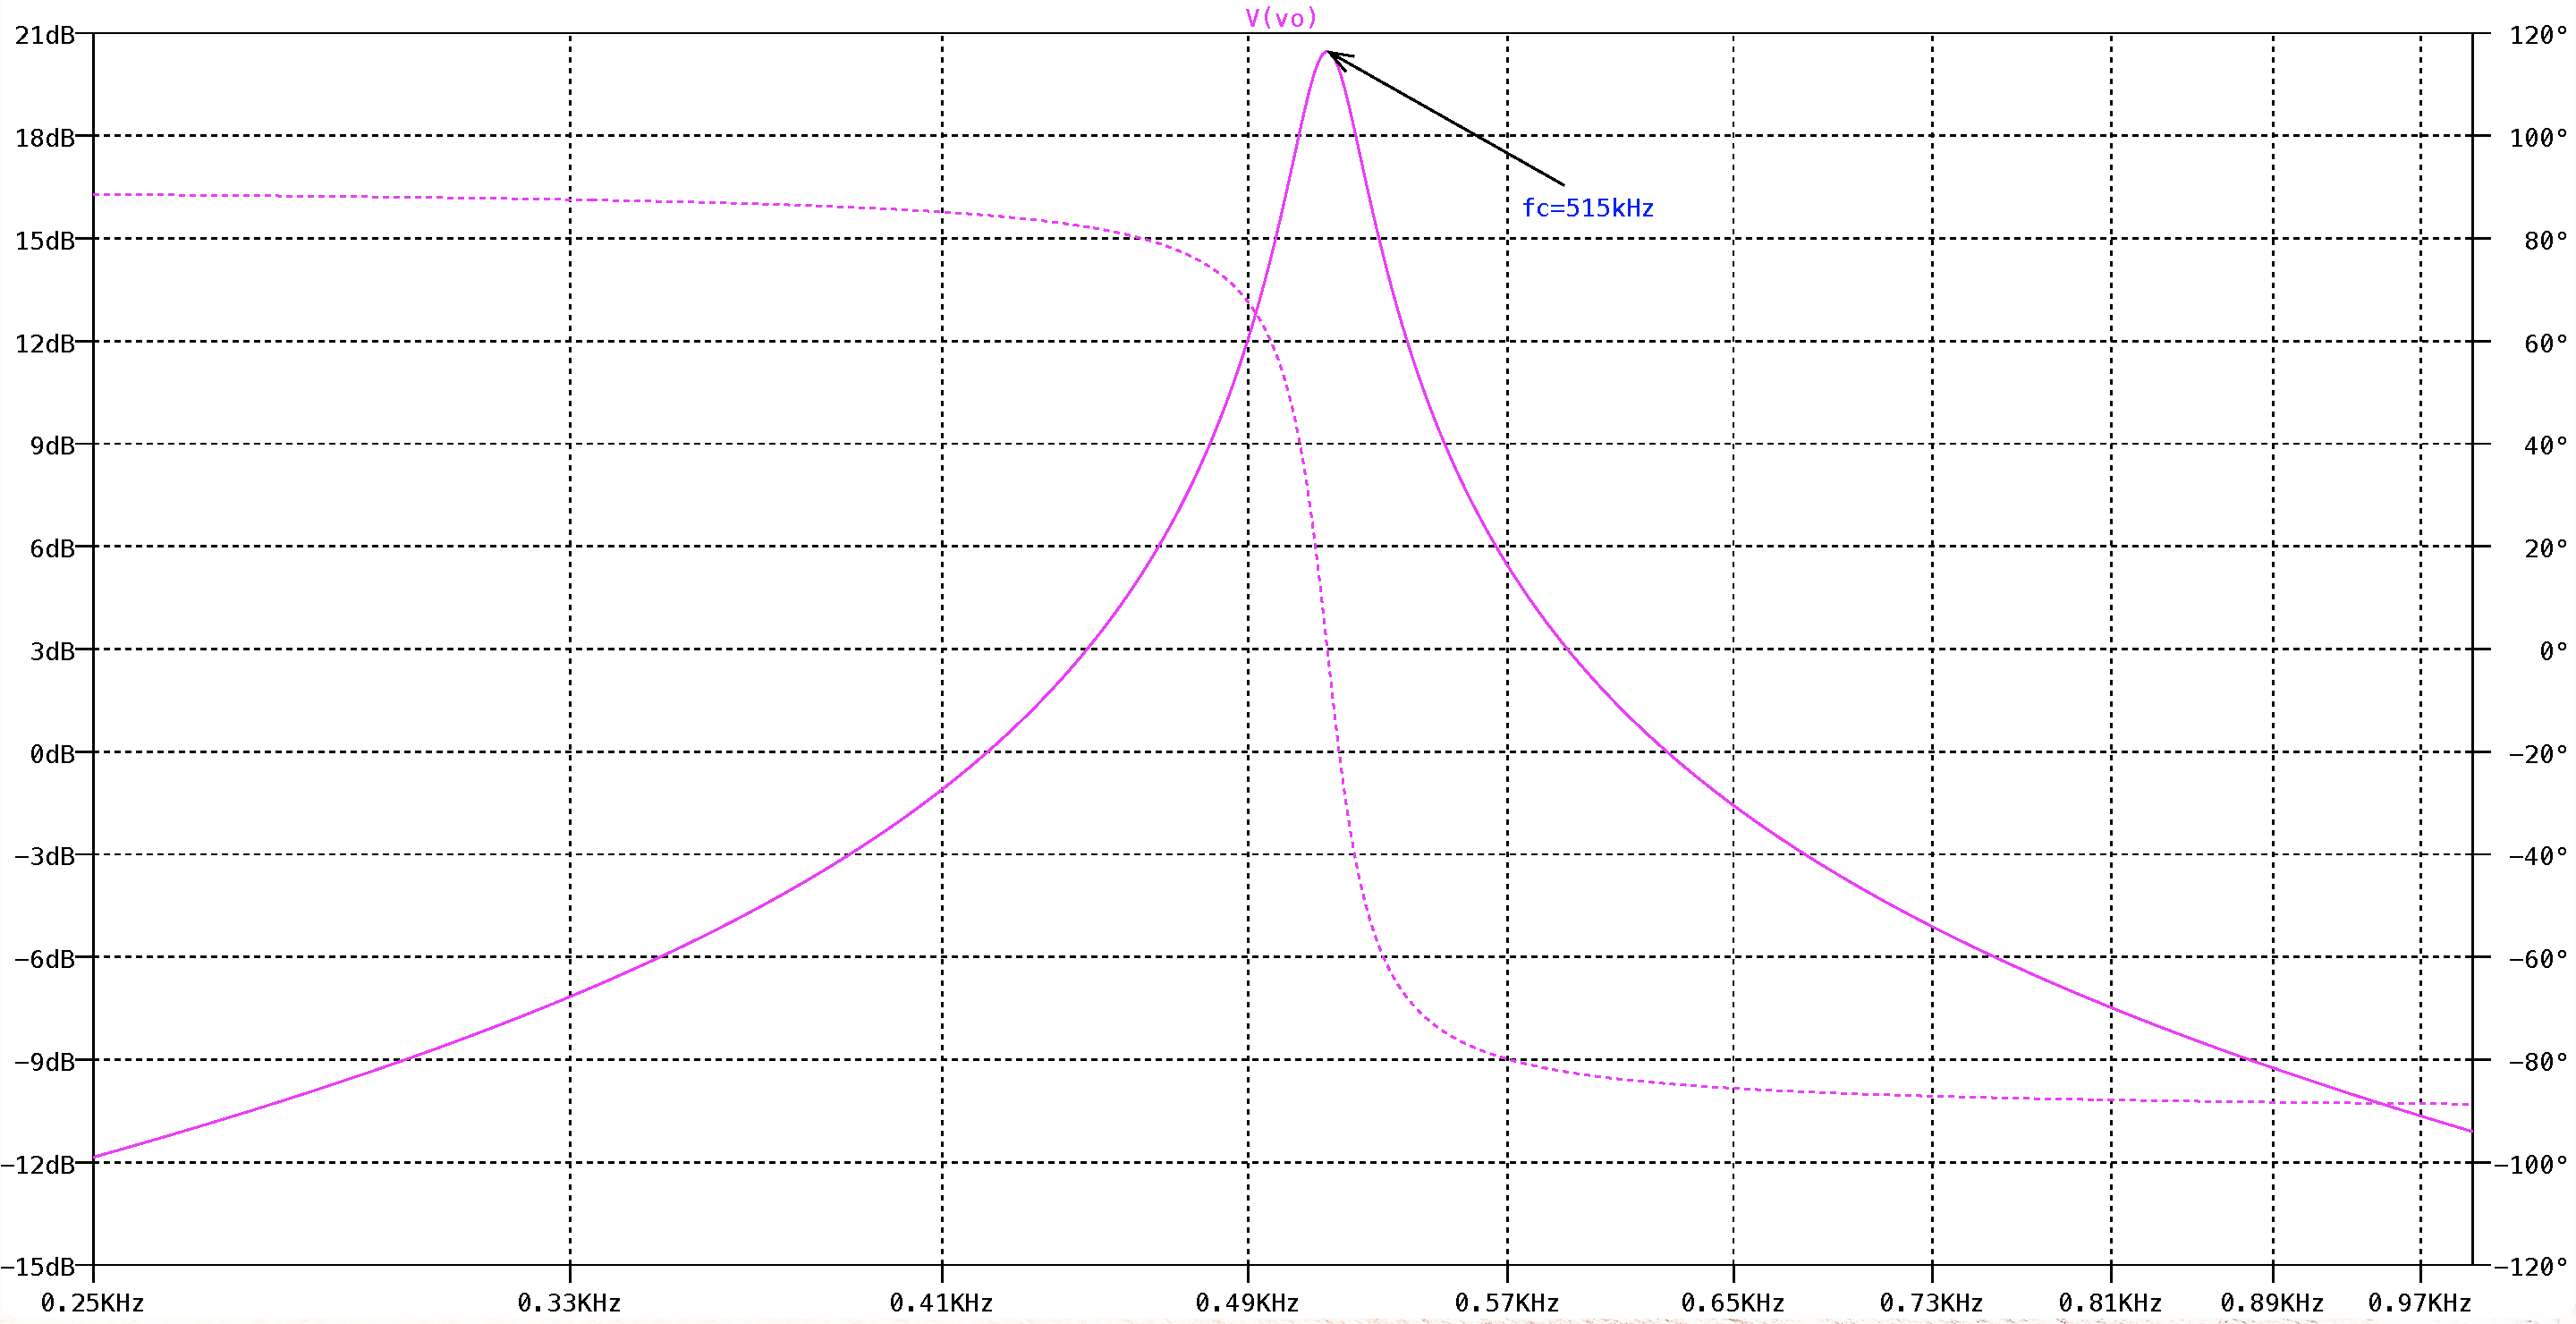
\includegraphics[width=0.65\textwidth]{Screenshots/q7_graph}  
	\caption{Three Op-Amp Biquad Band Pass Filter Graph}
	\label{q7_graph}
\end{figure}

\section*{Questions}

Step 2) The capacitor value was found to be 15.92 nF. \\

Step 3) The slope of each magnitude plot during the descent is -20 dB/dec.  \\

Step 4a) To keep $f_c$ unchanged, the R value of the previous stage is the R value of the final stage divided by a factor of 10, so it becomes 1 \si{\kilo\ohm}. The C value of the previous stage is the C value of the final stage multiplied by a factor of 10, so it becomes 100 nF. The new value of f(-3 dB) is 1023 Hz. \\

Step 4b) The same pattern continues, where the new R value is scaled down by a factor of 10 from the stage directly to the right of the new stage being added. This new R value is 100 \si{\ohm}. The C value is scaled up by a factor of 10 from the stage directly to the right of the new stage being added. The new C value is 1000 nF. The new value of f(-3 dB) is 811 Hz. \\

Step 4c) As more stages are added, this pattern continues, where R will continue to decrease by a factor of 10 and C will continue to increase by a factor of 10. \\

Step 4d) A voltage follower (op amp with a gain of 1) could be an ideal buffer between stages of the filter as its order continues to increase.

\newpage
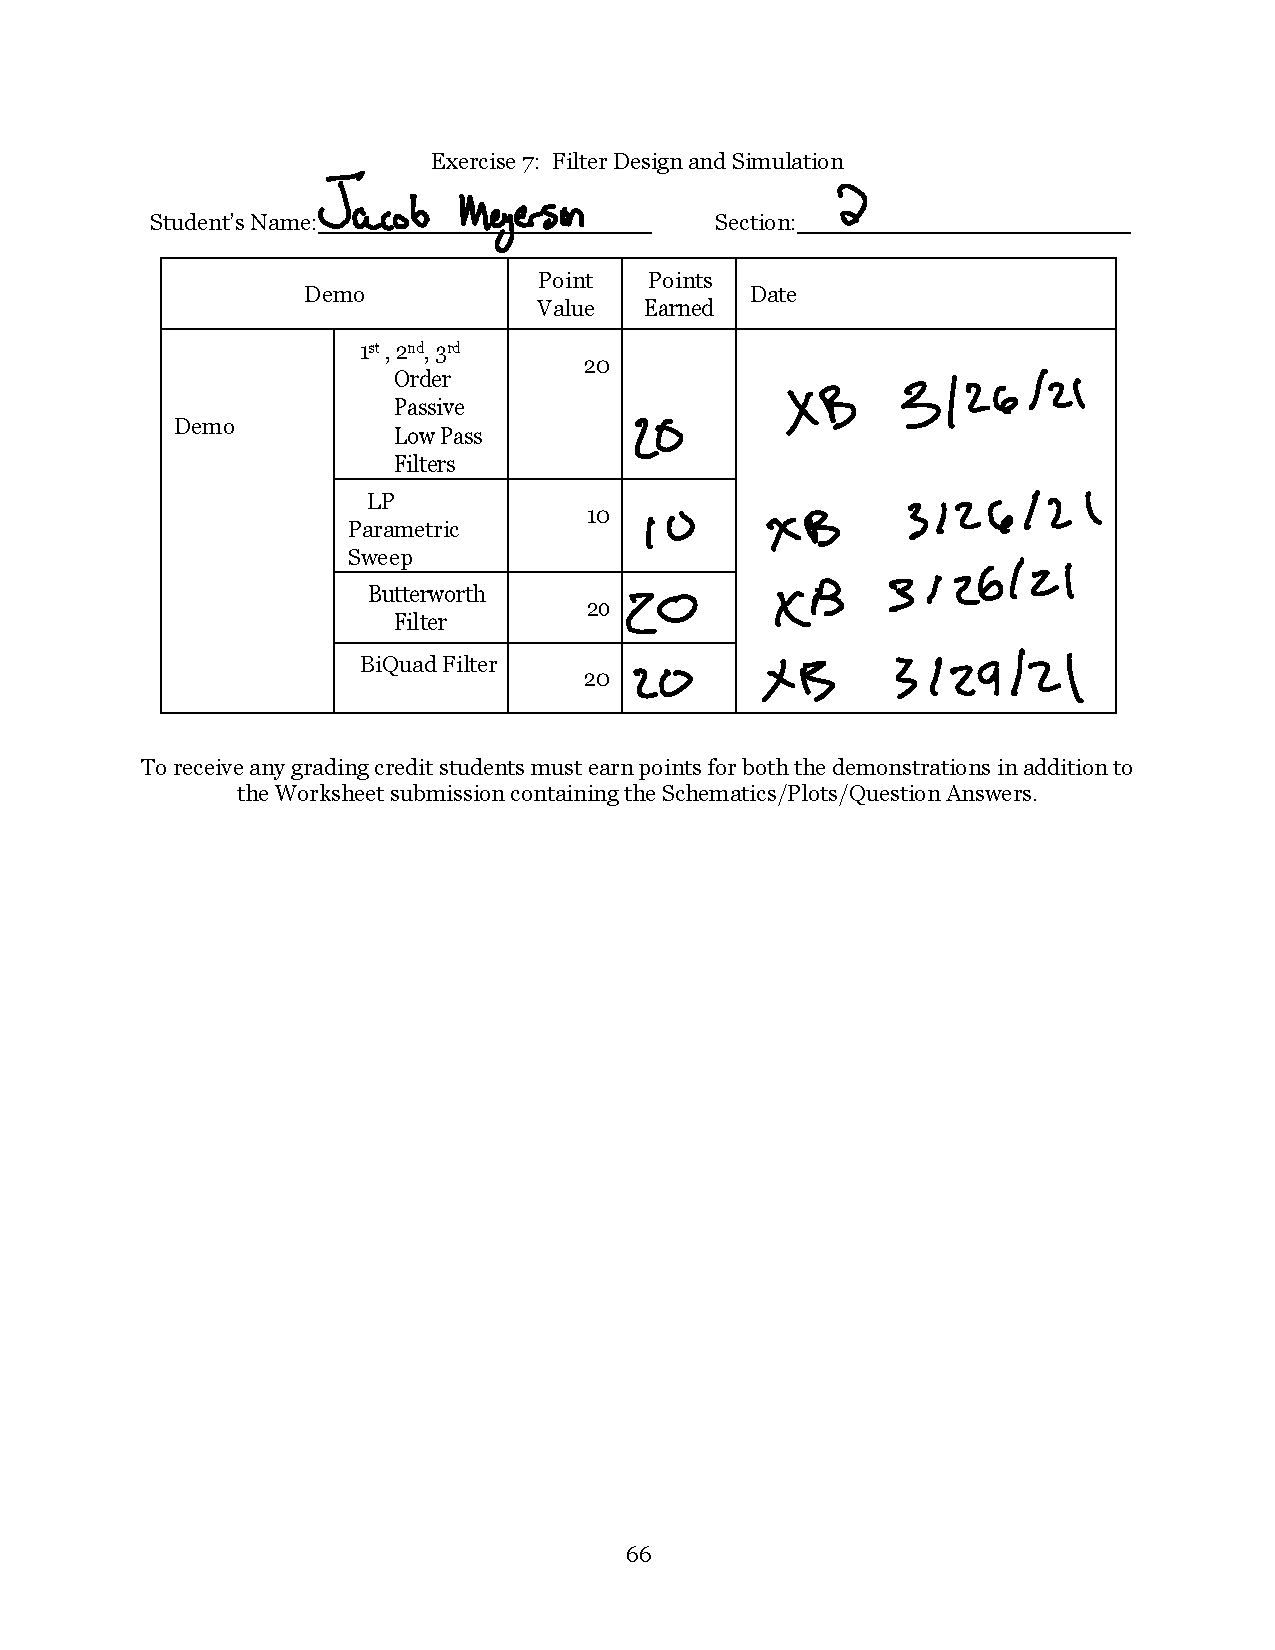
\includepdf[pages=-,pagecommand={},width=\paperwidth]{lab7_signoff.pdf}

\end{document}